\documentclass[a4paper]{article}
\usepackage[normalem]{ulem}
\usepackage{graphicx}
\usepackage[font=small,labelfont=bf]{caption}

% impostazioni generali
%Tutti gli usepackage vanno qui
\usepackage[table]{xcolor}
\usepackage{geometry}
\usepackage[italian]{babel}
\usepackage[utf8]{inputenc}
\usepackage{tabularx}
\usepackage{longtable}
\usepackage{hyperref}
\usepackage{enumitem}
\usepackage{array} 
\usepackage{booktabs}
\newcolumntype{M}[1]{>{\centering\arraybackslash}m{#1}}
\usepackage[toc]{appendix}
\usepackage{caption}

\hypersetup{
	colorlinks=true,
	linkcolor=blue,
	filecolor=magenta,
	urlcolor=blue,
}
% Numerazione figure
\let\counterwithout\relax
\let\counterwithin\relax
\usepackage{chngcntr}

% distanziare elenco delle figure e delle tabelle
\usepackage{tocbasic}
\DeclareTOCStyleEntry[numwidth=3.5em]{tocline}{figure}% for figure entries
\DeclareTOCStyleEntry[numwidth=3.5em]{tocline}{table}% for table entries


%\counterwithout{table}{section}
%\counterwithout{figure}{section}
\captionsetup[table]{font=small,skip=5pt} 

\usepackage[bottom]{footmisc}
\usepackage{fancyhdr}
\setcounter{secnumdepth}{4}
\usepackage{amsmath, amssymb}
\usepackage{array}
\usepackage{graphicx}

\usepackage{ifthen}

\usepackage{float}
\restylefloat{table}

\usepackage{layouts}
\usepackage{url}
\usepackage{comment}
\usepackage{eurosym}

\usepackage{lastpage}
\usepackage{layouts}
\usepackage{eurosym}

\geometry{a4paper,top=3cm,bottom=4cm,left=2.5cm,right=2.5cm}

%Comandi di impaginazione uguale per tutti i documenti
\pagestyle{fancy}
\lhead{
\includegraphics[scale=0.25]{template/images/logo-inline.png}}


%\rfoot{\thepage}
\cfoot{Pagina \thepage\ di \pageref{LastPage}}
\setlength{\headheight}{35pt}
\setcounter{tocdepth}{5}
\setcounter{secnumdepth}{5}
\renewcommand{\footrulewidth}{0.4pt}

% multirow per tabelle
\usepackage{multirow}

% Permette tabelle su più pagine
%\usepackage{longtable}


%COMANDI TABELLE
\newcommand{\rowcolorhead}{\rowcolor[HTML]{731733}}
\newcommand{\captionline}{\rowcolor[HTML]{FFFFFF}} %comando per le caption delle tabelle
\newcommand{\cellcolorhead}{\cellcolor[HTML]{007c95}}
\newcommand{\hlinetable}{\arrayrulecolor[HTML]{007c95}\hline}

%intestazione
% check for missing commands
\newcommand{\headertitle}[1]{\textbf{\color{white}#1}} %titolo colonna
\definecolor{pari}{HTML}{dcbac2}
\definecolor{dispari}{HTML}{f5f5f5}

% comandi \textit{Glossario}
\newcommand{\glo}{$_{G}$}
\newcommand{\glosp}{$_{G}$ }


%label custom
\makeatletter
\newcommand{\uclabel}[2]{%
	\protected@write \@auxout {}{\string \newlabel {#1}{{#2}{\thepage}{#2}{#1}{}} }%
	\hypertarget{#1}{#2}
}
\makeatother

%riportare pezzi di codice
\definecolor{codegray}{gray}{0.9}
\newcommand{\code}[1]{\colorbox{codegray}{\texttt{#1}}}

% dati relativi alla prima pagina
\makeindex
\begin{document}
\counterwithin{table}{section}

% Prima pagina
\thispagestyle{empty}
\renewcommand{\arraystretch}{1.3}


\begin{titlepage}
	\begin{center}
		
	
\includegraphics[scale = 0.7]{template/images/logo-circle.png}
	\\[1cm]
	\href{mailto:6bitbusters@gmail.com}		      	
	{\large{\textit{6bitbusters@gmail.com} } }\\[1cm]
	
	\Huge \textbf{Analisi dei requisiti} \\[1cm]

	% Informazioni sul documento
	\large \textbf{Informazioni sul documento} \\
	\rule{0.6\textwidth}{0.4pt}
	\\[0.5cm]
	\begin{tabular}{r|l}
		\textbf{Versione} & 0.8.0\\
		\textbf{Stato} & in redazione\\
		\textbf{Uso} & esterno\\                         
		\textbf{Approvazione} & -\\                      
		\textbf{Redazione} & Pincin Matteo\\ & Diviesti Filippo\\ & Soranzo Andrea \\ & Djossa Edgar \\
		\textbf{Verifica} & Bergamin Elia\\ & Soranzo Andrea \\ & Chilese Elena \\  & Djossa Edgar \\                     
		\textbf{Distribuzione} & \parbox[t]{5cm}{ \textit{Six Bit Busters} \\ Prof. Vardanega Tullio 
	 \\ Prof. Cardin Riccardo}
	\end{tabular}	
	\\[1.2cm]

 % Descrizione
	\large \textbf{Descrizione} \\ Documento di rendicontazione dell'\textit{Analisi dei requisiti}
	
	
	\end{center}
\end{titlepage}


% Diario delle modifiche

\section*{Registro delle modifiche}

\newcommand{\changelogTable}[1]{

\renewcommand{\arraystretch}{1.5}
\rowcolors{2}{pari}{dispari}
\begin{longtable}{ %0.87
		>{\centering}M{0.10\textwidth} 
		>{\centering}M{0.11\textwidth}
		>{\centering}M{0.19\textwidth}
		>{\centering}M{0.28\textwidth} 
		>{\centering\arraybackslash}M{0.19\textwidth} 
		 }
	\rowcolorhead
	\headertitle{Versione} &
	\centering \headertitle{Data} &	
	\headertitle{Autore} &
	\headertitle{Descrizione} & 
	\headertitle{Verificatore} 
	\endfirsthead	
	\endhead
	
	#1

\end{longtable}
\vspace{-2em}

}
% Insert changelog values here
\changelogTable{
  2.0.1 & 19-03-2025 & Soranzo Andrea & Rimossi numeri di sezione & - \tabularnewline
  2.0.0 & 02-03-2025 & Soranzo Andrea & Approvazione documento & - \tabularnewline
	1.1.0 & 02-03-2025 & Bergamin Elia & Integrazione vocaboli & Djossa Edgar \tabularnewline
	1.0.0 & 31-01-2025 & Soranzo Andrea & Approvazione documento & - \tabularnewline
	0.7.0 & 30-01-2025 & Chilese Elena & Revisione documento & Bergamin Elia \tabularnewline
	0.6.0 & 28-01-2025 & Bergamin Elia & Integrazione vocaboli & Pincin Matteo \tabularnewline
	0.5.0 & 10-01-2025 & Diviesti Filippo & Integrazione vocaboli & Soranzo Andrea\tabularnewline
    0.4.0 & 16-12-2024 & Djossa Edgar & Integrazione vocaboli & Chilese Elena \tabularnewline   
	0.3.0 & 10-12-2024 & Bergamin Elia & Aggiunta Introduzione, integrazione vocaboli e morfologia & Djossa Edgar \tabularnewline
	0.2.0 & 25-11-2024 & Bergamin Elia & Integrazione vocaboli & Soranzo Andrea \tabularnewline
	0.1.0 & 19-11-2024 & Diviesti Filippo & Inserimento vocaboli per \textit{Norme di progetto} e \textit{Piano di progetto} & Pincin Matteo \\
}

\pagebreak

% Indice
{
    \hypersetup{linkcolor=black}
    \tableofcontents
}
\pagebreak

\hypersetup{colorlinks=false, linkcolor=black}
\listoffigures
\hypersetup{colorlinks=true, linkcolor=blue}

% Contenuto
\section{Introduzione}
\subsection{Scopo del documento}
Questo documento ha lo scopo di descrivere le scelte progettuali fondamentali
per la struttura, il comportamento e l'interoperabilità del sistema software.
In particolare, serve a:
\begin{itemize}
      \item Definire i moduli, le componenti, le loro responsabilit`a e le interazioni;
      \item Fornire un riferimento agli sviluppatori per implementare il software in modo
            coerente;
      \item Garantire la completa copertura dei requisiti individuati nell'\textit{Analisi
                  dei requisiti v2.0.0}.
\end{itemize}
A tale scopo, il documento descrive le tecnologie selezionate, l'architettura implementativa e l'architettura
di deployment. Ciò include la descrizione delle classi, dei design pattern e delle librerie utilizzate, anche
con l'ausilio di diagrammi UML.

\subsection{Scopo del prodotto}
\textit{3Dataviz} è un prodotto ideato dall'azienda \textit{Sanmarco Informatica S.p.A.} per semplificare e rendere più accessibile la visualizzazione dei dati.\\
Esso mira a trasformare i dati in grafici e rappresentazioni visive, sfruttando la capacità del cervello umano di elaborare rapidamente le immagini.
Questo approccio facilita il processo decisionale e migliora la comprensione delle informazioni.\\
L'obiettivo principale è lo sviluppo di un'interfaccia web che trasforma dati provenienti da diverse fonti (come database e REST API) in grafici 3D interattivi e navigabili.
I dati potranno essere consultati anche in formato tabellare, offrendo una visione alternativa ma altrettanto utile.

\subsection{Glossario}
Per chiarire i termini tecnici o ambigui si utilizza un glossario disponibile
nel file \textit{Glossario v2.0.0}.\\ Tutti i termini che richiedono
spiegazioni sono indicati con il pedice “g”. \\ Questa convenzione consente un
rapido collegamento tra il testo e la relativa spiegazione dettagliata nel
glossario, garantendo coerenza e chiarezza.

\subsection{Riferimenti normativi}
\begin{itemize}
      \item \textit{Norme di progetto v2.0.0} \\ \url{https://6bitbusters.github.io/norme_di_progetto.pdf}
      \item Capitolato d'appalto C5 - \textit{Sanmarco Informatica S.p.A.}: 3Dataviz \\
            \url{https://www.math.unipd.it/~tullio/IS-1/2024/Progetto/C5.pdf}
\end{itemize}

\subsection{Riferimenti informativi}
\begin{itemize}
      \item Slide T6 - Corso di Ingegneria del Software - Progettazione software: \\
            \url{https://www.math.unipd.it/~tullio/IS-1/2024/Dispense/T06.pdf}
      \item Slide P - Corso di Ingegneria del Software - Diagrammi delle classi: \\
            \url{https://www.math.unipd.it/~rcardin/swea/2023/Diagrammi%20delle%20Classi.pdf}
\end{itemize}

\pagebreak

% insert here other content (\include)
\section{Tecnologie}
Questa sezione descrive gli strumenti e le tecnologie adottati per lo sviluppo,
il testing e il deployment del software relativo al progetto \textit{3Dataviz}.
In particolare, vengono illustrati il linguaggio di programmazione, le
librerie, i framework e le infrastrutture utilizzate.

\subsection{Linguaggio di programmazione}
\subsubsection{TypeScript}
TypeScript è un linguaggio di programmazione open-source sviluppato da
Microsoft. Si tratta di un superset di JavaScript, che introduce la
tipizzazione statica, consentendo di rilevare errori di programmazione in fase
di sviluppo, ridurre il numero di bug e migliorare la qualità del codice.
\begin{itemize}
    \item \textbf{Versione}: 5.8.2;
    \item \textbf{Documentazione}: \url{https://www.typescriptlang.org/docs/} (consultato:
          25-03-2025).
\end{itemize}
Nel contesto del progetto \textit{3Dataviz}, TypeScript è il linguaggio principale
utilizzato per lo sviluppo sia del frontend che del backend. \\Per il frontend,
si utilizza TSX, un'estensione di Typescript che permette di definire la struttura
dell'interfaccia utente in modo più leggibile e dichiarativo, integrando HTML
direttamente nel codice TypeScript.

\subsection{Formato dei dati}
\subsubsection{JSON}
JSON (JavaScript Object Notation) è un formato di scambio dati leggero e
indipendente dal linguaggio di programmazione. È ampiamente utilizzato nello
sviluppo web e nello scambio di dati tra applicazioni. \\JSON è basato su due
strutture di dati:
\begin{itemize}
    \item \textbf{Oggetti}: insiemi di coppie chiave-valore;
    \item \textbf{Array}: liste ordinate di valori.
\end{itemize}
JSON viene utilizzato per la trasmissione dei dati tra frontend e backend, nonché
per la memorizzazione dei dati nel sistema di cache.

\subsection{Frontend}
\subsubsection{Vite}
Vite è uno strumento di build progettato per offrire un'esperienza di sviluppo
veloce e fluida nei progetti web moderni. Si compone di due parti principali:
\begin{itemize}
    \item Un server di sviluppo, che estende le funzionalità dei moduli ES nativi,
          offrendo, ad esempio, un Hot Module Replacement (HMR) estremamente rapido;
    \item Un comando di compilazione che crea il bundle del codice utilizzando Rollup,
          preconfigurato per generare risorse statiche ottimizzate per la produzione.
\end{itemize}
Vite è estendibile tramite plugin, che consentono di personalizzare
il processo di sviluppo e di compilazione. Nel progetto \textit{3Dataviz}, viene utilizzato il
plugin \texttt{@vitejs/plugin-react-swc}, che abilita la sintassi JSX e ottimizza la compilazione del codice React.

\begin{itemize}
    \item \textbf{Versione}: 6.2.3;
    \item \textbf{Documentazione}: \url{https://vitejs.dev/guide/} (consultato:
          25-03-2025).
\end{itemize}

\subsubsection{Three.js}
Three.js è una libreria JavaScript open-source per la creazione di grafica 3D.
Fornisce un'API ad alto livello per la creazione di scene 3D complesse,
utilizzando WebGL come backend per la grafica hardware-accelerata. \\Three.js
semplifica la creazione di oggetti 3D, luci, materiali e animazioni, offrendo
funzionalità avanzate come il ray tracing e il supporto per shading e texture.
\begin{itemize}
    \item \textbf{Versione}: 0.174.0;
    \item \textbf{Documentazione}: \url{https://threejs.org/docs/} (consultato:
          25-03-2025).
\end{itemize}
Questa è la libreria intorno su cui si basa l'intero progetto, in quanto
viene utilizzata per la visualizzazione dei dati in 3D, nonché per la
navigazione e l'interazione con il grafico.

\subsubsection{GSAP}
GSAP (GreenSock Animation Platform) è una libreria JavaScript open-source per
la creazione di animazioni di alta qualità.
\begin{itemize}
    \item \textbf{Versione}: 3.12.7;
    \item \textbf{Documentazione}: \url{https://gsap.com/docs/v3} (consultato:
          25-03-2025).
\end{itemize}
GSAP è necessaria per l'implementazione dei casi d'uso relativi al posizionamento
della camera in punti specifici della scena 3D, nonché per la gestione delle
animazioni di transizione tra un punto e l'altro.

\subsubsection{React}
React è una libreria JavaScript open-source per la creazione di interfacce
utente. Consente di definire componenti riutilizzabili che rappresentano parti
dell'interfaccia, aggiornando automaticamente la vista in base allo stato
dell'applicazione. \\React adotta un approccio dichiarativo per la definizione
dell'interfaccia utente, semplificando la gestione dello stato e la
sincronizzazione con il DOM. \\Non è opinionato nella scelta delle librerie di
routing o di gestione dello stato, permettendo una facile integrazione con
altre tecnologie.
\begin{itemize}
    \item \textbf{Versione}: 19.0.0;
    \item \textbf{Documentazione}: \url{https://react.dev/learn} (consultato:
          25-03-2025).
\end{itemize}

\paragraph{React Router}
Libreria open-source che fornisce un sistema di routing per React. Consente di
definire rotte all'interno dell'applicazione, associando componenti React a URL
specifici. \\React Router gestisce la navigazione tra le diverse rotte,
aggiornando il contenuto dell'interfaccia utente in base all'URL corrente.
\begin{itemize}
    \item \textbf{Versione}: 7.4.0;
    \item \textbf{Documentazione}: \url{https://reactrouter.com/home} (consultato:
          25-03-2025).
\end{itemize}

\paragraph{React Three Fiber}
Libreria open-source che permette di integrare Three.js all'interno di
un'applicazione React. Fornisce un'API dichiarativa per la creazione di scene
3D, semplificando l'integrazione di Three.js con React e consentendo di
definire componenti 3D riutilizzabili.
\begin{itemize}
    \item \textbf{Versione}: 9.1.0;
    \item \textbf{Documentazione}: \url{https://docs.pmnd.rs/react-three-fiber/getting-started/introduction} (consultato:
          25-03-2025).
\end{itemize}

\paragraph{React Three Drei}
Libreria open-source che fornisce componenti e hook riutilizzabili per React
Three Fiber. Contiene una vasta gamma di componenti pronti all'uso per la
creazione di scene 3D, semplificando lo sviluppo di applicazioni 3D basate su
React e Three.js.
\begin{itemize}
    \item \textbf{Versione}: 10.0.5;
    \item \textbf{Documentazione}: \url{https://drei.docs.pmnd.rs/getting-started/introduction} (consultato:
          25-03-2025).
\end{itemize}

\subsubsection{Redux}
Redux è una libreria open-source per la gestione dello stato globale nelle
applicazioni JavaScript. Si basa su due concetti fondamentali:
\begin{itemize}
    \item \textbf{Store}, che rappresenta lo stato dell'applicazione;
    \item \textbf{Azioni}, che definiscono le modifiche allo stato.
\end{itemize}
Redux semplifica la gestione dello stato, fornendo un'API per definire
azioni e reducer, che aggiornano lo stato in base alle azioni ricevute.
\begin{itemize}
    \item \textbf{Versione}: 5.0.1;
    \item \textbf{Documentazione}: \url{https://redux.js.org/introduction/getting-started} (consultato:
          25-03-2025).
\end{itemize}
Redux è utilizzato per gestire lo stato globale dell'applicazione, in particolare per
memorizzare i dati caricati dal backend e per gestire lo stato della
visualizzazione 3D.

\paragraph{Redux Toolkit}
Pacchetto ufficiale per Redux, progettato per semplificare la gestione dello
stato. Viene utilizzato per configurare lo store Redux e per definire le azioni
e i reducer necessari alla gestione dello stato globale dell'applicazione.
\begin{itemize}
    \item \textbf{Versione}: 2.6.1;
    \item \textbf{Documentazione}: \url{https://redux-toolkit.js.org/introduction/getting-started} (consultato:
          25-03-2025).
\end{itemize}

\paragraph{React Redux}
Pacchetto che funge da collegamento tra l'interfaccia utente in React e Redux.
Consente ai componenti React di leggere i dati dallo store Redux e di inviare
azioni per aggiornare lo stato dell'applicazione.
\begin{itemize}
    \item \textbf{Versione}: 9.2.0;
    \item \textbf{Documentazione}: \url{https://react-redux.js.org/introduction/getting-started} (consultato:
          25-03-2025).
\end{itemize}

\subsubsection{Axios}
Axios è un client HTTP basato su Promise per Node.js e browser. È isomorfo,
cioè può essere eseguito sia nel browser che in Node.js utilizzando lo stesso
codice sorgente. Lato server, Axios utilizza il modulo http nativo di Node.js,
mentre lato client usa XMLHttpRequest.
\begin{itemize}
    \item \textbf{Versione}: 1.8.4;
    \item \textbf{Documentazione}: \url{https://axios-http.com/docs/intro} (consultato:
          25-03-2025).
\end{itemize}
Nel progetto \textit{3Dataviz}, Axios viene utilizzato:
\begin{itemize}
    \item Lato frontend, per effettuare richieste HTTP al backend e ottenere i dati da
          visualizzare nel grafico 3D;
    \item Lato backend, per effettuare richieste HTTP alle API esterne, acquisendo i dati
          da elaborare e inviare al frontend.
\end{itemize}

\subsection{Backend}
\subsubsection{Node.js}
Node.js è un runtime JavaScript open-source basato sul motore V8 di Google
Chrome. Consente di eseguire codice JavaScript lato server, utilizzando un
modello di I/O asincrono e orientato agli eventi. Node.js è progettato per
essere leggero e scalabile, adatto per la creazione di applicazioni web ad alte
prestazioni.
\begin{itemize}
    \item \textbf{Versione}: 22.14.0;
    \item \textbf{Documentazione}: \url{https://nodejs.org/en/docs/} (consultato:
          25-03-2025).
\end{itemize}

\subsubsection{NestJS}
NestJS è un framework per Node.js che fornisce un'architettura modulare e
scalabile per la creazione di applicazioni lato server. \\Si basa su
Express.js, offrendo funzionalità aggiuntive come la dependency injection, i
middleware e i decorator. NestJS consente di organizzare il codice in moduli
riutilizzabili e di definire facilmente controller, servizi e provider.
\begin{itemize}
    \item \textbf{Versione}: 11.0.12;
    \item \textbf{Documentazione}: \url{https://docs.nestjs.com/} (consultato:
          26-03-2025).
\end{itemize}
Nel progetto \textit{3Dataviz}, NestJS è utilizzato per creare il backend,
definendo i controller per gestire le richieste HTTP effettuate dal frontend,
i servizi per ottenere ed elaborare i dati provenienti dalle API esterne, e i
provider per l'iniezione delle dipendenze.

\subsubsection{Memcached}
Memcached è un sistema di cache open-source ad alte prestazioni, progettato per
accelerare le applicazioni web dinamiche alleggerendo il carico del database.
Funziona come un archivio chiave-valore per piccoli dati arbitrari (massimo 1
MB) che possono consistere in risultati di chiamate a database o a API.
\begin{itemize}
    \item \textbf{Versione}: 1.6.38;
    \item \textbf{Documentazione}: \url{https://docs.memcached.org/} (consultato:
          26-03-2025).
\end{itemize}
Memcached viene utilizzato per memorizzare i dati ottenuti dalle API esterne,
al fine di ridurre i tempi di accesso ai dati, nonché il numero di richieste
effettuate alle API. Ciò è particolarmente utile nel caso di API che impongono
un limite massimo di richieste per unità di tempo.

\subsection{Deployment}
\subsubsection{Docker}
Docker è una piattaforma open-source per lo sviluppo, la distribuzione e
l'esecuzione di applicazioni in contenitori. I contenitori Docker sono unità
standardizzate di software che includono il codice sorgente, le dipendenze e le
configurazioni necessarie per eseguire un'applicazione.
\begin{itemize}
    \item \textbf{Documentazione}: \url{https://docs.docker.com/} (consultato:
          26-03-2025).
\end{itemize}
Per lo sviluppo, il testing e il rilascio del prodotto sono stati utilizzati container Docker in
modo da garantire ambienti consistenti e riproducibili.

\subsection{Testing}
\subsubsection{Vitest}
Vitest è un framework di testing per Vite. Offre funzionalità avanzate come il
supporto per TypeScript, la configurazione tramite file di setup e la
possibilità di eseguire test in modalità watch. Questa è particolarmente utile
in fase di sviluppo attivo e debugging, poiché riduce i tempi di attesa per
l'esecuzione dei test e aiuta a mantenere il codice sempre funzionante durante
il processo di sviluppo.
\begin{itemize}
    \item \textbf{Versione}: 3.0.9;
    \item \textbf{Documentazione}: \url{https://vitest.dev/guide/} (consultato:
          26-03-2025).
\end{itemize}
Vitest è utilizzato per eseguire i test di unità e di integrazione del frontend,
verificando che i componenti React siano implementati correttamente.

\subsubsection{Cypress}
Cypress è un framework di testing end-to-end per applicazioni web. Consente di
scrivere test in JavaScript, eseguirli in un browser reale e visualizzare i
risultati in tempo reale.
\begin{itemize}
    \item \textbf{Versione}: 14.2.0;
    \item \textbf{Documentazione}: \url{https://docs.cypress.io/} (consultato:
          26-03-2025).
\end{itemize}
Cypress è utilizzato per testare il frontend dell'applicazione, verificando che
l'interfaccia utente sia correttamente visualizzata e che le principali funzionalità
siano implementate correttamente.

\subsubsection{Jest}
Jest è un framework di testing progettato per garantire la correttezza di
qualsiasi sorgente JavaScript. Consente di scrivere test con un'API
accessibile e ricca di funzionalità che fornisce risultati rapidamente.
\begin{itemize}
    \item \textbf{Versione}: 29.7.0;
    \item \textbf{Documentazione}: \url{https://jestjs.io/docs/getting-started} (consultato:
          26-03-2025).
\end{itemize}
Jest è utilizzato per eseguire i test di unità e di integrazione del backend,
verificando che i servizi e i controller siano implementati correttamente.
\pagebreak

\section{Descrizione dell'architettura}
\subsection{Architettura frontend}
\subsubsection{Design pattern architetturale}

\paragraph{Redux-Toolkit}
I componenti che costituiscono l'architettura frontend utilizzata seguono il
pattern offerto dalla libreria Redux-Toolkit. Redux-Toolkit è pensato per
integrarsi con React e consente di gestire i dati condivisi tra i componenti React in modo centralizzato,
semplificando la gestione dello stato globale dell'applicazione. Inoltre
Redux-Toolkit è un wrapper che semplifica l'utilizzo di Redux in modo tale da
scrivere meno codice e commettere meno errori durante lo sviluppo.

I componenti che formano l'architettura di Redux-Toolkit sono:
\begin{itemize}
    \item \textbf{Store:} componente che contiene lo stato globale dell'applicazione.
          All'avvio dell'applicazione viene configurato utilizzando RootReducer e i componenti che utilizzano
          lo stato globale si mettono in ascolto dello store in modo da venire renderizzati ogni volta che un dato
          di interesse cambia valore. Questo modo di operare può essere visto come un pattern Observer in
          cui lo store è il Subject e gli Observer sono i componenti React che osservano i cambiamenti dello store;
    \item \textbf{RootReducer:} componente utilizzato per configurare lo store combinando le slice;
    \item \textbf{Slice:} componente che contiene un proprio stato che rappresenta una porzione dello stato globale
          dell'applicazione, i reducer che operano su tale stato e i selector per consentire ai suoi client il
          reperimento dei dati;
    \item \textbf{Reducer:} componente che riceve come parametri uno stato iniziale (InitialState) e un'action
          (composta da un type e un payload) e restituisce lo stato dopo aver operato sui dati.
          Il type rappresenta una stringa univoca che ha lo scopo di identificare la specifica action che si intende eseguire.
          Il payload è un oggetto che contiene i dati necessari per l'esecuzione dell'action.
          React-Toolkit gestisce le chiamate ai reducer in seguito ai dispatch delle action che avvengono
          specificando solamente l'oggetto che rappresenta il payload;
          Con il termine dispatch si intende una funzione che viene chiamata per inviare una action allo store di Redux e innescare un cambiamento dello stato.
    \item \textbf{Action:} oggetto composto da un type e da un payload di cui viene effettuato il dispatch quando
<<<<<<< HEAD
    opportuno.
    \item \textbf{State:} componente che contiene i dati di una slice su cui essa opera.
    Importante sottolineare che Redux-Toolkit garantisce l’immutabilità dei dati in modo che i reducer restituiscano delle copie dello stato in modo che esso non possa venire
    modificato dall’esterno è utilizzato in modo improprio.
    L’unico modo per modificare i dati dello stato globale `e quindi con il dispatch di un’action;
=======
          opportuno. Il payload è un oggetto che contiene i dati da passare al reducer che catturerà l'action;
    \item \textbf{InitialState:} componente che contiene i dati di una slice su cui essa opera.
          Importante sottolineare che Redux-Toolkit garantisce l'immutabilità dei dati in modo che i reducer restituiscano delle copie dello stato in modo che esso non possa venire
          modificato dall'esterno è utilizzato in modo improprio.
          L'unico modo per modificare i dati dello stato globale è quindi con il dispatch di un'action;
>>>>>>> 7cc2534ef4700ebec7c9c79a5a0841bc32c1a5fe
    \item \textbf{Selector:} funzione che prende lo stato corrente di una slice come argomento e ritorna un sottoinsieme
          specifico del suo stato. In altre parole, un selector consente di selezionare una parte specifica
          dello stato in modo da poterla utilizzare in modo isolato all'interno di un componente React.
\end{itemize}

\subsubsection{Elenco dei componenti}
<<<<<<< HEAD
Poiché il team di sviluppo frontend utilizzerà Redux per la gestione dello stato, l'applicazione sarà strutturata principalmente attraverso la suddivisione del codice in slice, state e action.
=======
Poiché il team di sviluppo frontend utilizzerà Redux per la gestione dello
stato, l'applicazione sarà strutturata principalmente attraverso la
suddivisione del codice in slice, stati iniziali e action.
>>>>>>> 7cc2534ef4700ebec7c9c79a5a0841bc32c1a5fe
\paragraph{Slice}
Le slice contengono una porzione dello stato globale dell'applicazione che è
gestita da un reducer specifico.
\begin{itemize}
    \item \textbf{DataSlice:} componente che gestisce lo stato e contiene i dati relativi al dataset selezionato dall'utente;
    \item \textbf{AppStateSlice:} componente che gestisce lo stato dell'applicazione come errori e caricamenti;
    \item \textbf{DataSourceSlice:} componente che gestisce lo stato e contiene l'elenco dei dataset selezionabili dall'utente e il dataset selezionato;
    \item \textbf{FilterOptionSlice:} componente che gestisce lo stato e contiene le opzioni di filtraggio dei valori;
    \item \textbf{ViewOptionSlice:} componente che gestisce lo stato e contiene le opzioni di visibilità del piano medio;
    \item \textbf{RaycastHitSlice:} componente che gestisce lo stato e contiene le informazioni relative al raycast.
\end{itemize}
<<<<<<< HEAD
\paragraph{State}
    Gli state, definiti all'interno di ciascuna slice, si combinano per formare lo stato globale iniziale, gestito dallo store.
    \begin{itemize}
        \item \textbf{DataState:} componente che contiene i dati relativi al dateset selezionato dall'utente;
        \item \textbf{AppState:} componente che contiene i dati relativi allo stato attuale dell'applicazione;
        \item \textbf{DataSourceState:} componente che contiene le informazioni principali di tutti i dataset e quelle relative al dataset selezionato dall'utente;
        \item \textbf{FilterOptionState:} componente che contiene i dati relativi alle opzioni di filtraggio selezionate dall'utente;
        \item \textbf{ViewOptionState:} componente che contiene i dati relativi alle opzioni di visibilità del piano medio all'interno dell'ambiente 3D;
        \item \textbf{RaycastHitState:} componente che contiene i dati relativi al raycast, utilizzati per l'interazione con le barre del grafico 3D.
    \end{itemize}
\paragraph{Action}
    Le action, emesse dai componenti, vengono inviate ai reducer per aggiornare lo stato corrispondente.
    Ogni action è caratterizzata da un type e da un payload, che viene utilizzato dalle slice per modificare lo stato.
    Per convenzione il nome delle action segue il formato: \\
    \begin{center}
        \textbf{[nome slice].[nome funzione]}.
    \end{center}
    \begin{itemize}
        \item \textbf{DataSlice.requestData:} action asincrona emessa per recuperare dal server i dati del dataset selezionato; \\ Payload: nessuno
        \item \textbf{DataSlice.filterTopN:} action emessa per filtrare i dati, visualizzando esclusivamente i primi N valori più alti o più bassi; \\ Payload: FilterPayload
        \item \textbf{DataSlice.filterAboveValue:} action emessa per filtrare i dati, visualizzando esclusivamente quelli con un valore maggiore o minore rispetto al valore della barra del grafico selezionata;\\ Payload: FilterPayload
        \item \textbf{DataSlice.filterAverage:} action emessa per filtrare i dati, visualizzando esclusivamente quelli con un valore maggiore o minore rispetto alla media globale; \\ Payload: boolean $\rightarrow$ maggiore o minore
        \item \textbf{AppStateSlice.setLoading:} action emessa per aggiornare lo stato dell'applicazione e visualizzare la pagina di caricamento; \\ Payload: boolean
        \item \textbf{AppStateSlice.setError:} action emessa per aggiornare lo stato dell'applicazione e visualizzare una schermata di errore specifica, basata sull'errore generato dall'applicazione; \\ Payload: number $\rightarrow$ codice di errore.
        \item \textbf{DataSourceSlice.requestDatasets:} action asincrona emessa per recuperare l'elenco delle informazioni relative a tutti i dataset disponibili; \\ Payload: nessuno.
        \item \textbf{DataSourceSlice.setCurrentDataset:} action emessa per aggiornare il dataset selezionato dall'utente; \\ Payload: number $\rightarrow$ ID del dataset.
        \item \textbf{ViewOptionSlice.toggleAveragePlane:} action emessa per aggiornare il flag di visibilità del piano medio globale nell'ambiente 3D; \\ Payload: boolean 
        \item \textbf{FilterOptionSlice.toggleIsGreater:} action emessa per aggiornare il flag che determina se il filtraggio deve essere eseguito per valori maggiori o minori; \\ Payload: boolean
        \item \textbf{RaycastHitSlice.setHit:} action emessa per aggiornare la barra selezionata nel grafico 3D; \\ Payload: number $\rightarrow$ ID della barra.
        \item \textbf{RaycastHitSlice.setTooltipPosition:} action emessa per aggiornare la posizione del tooltip in base alla posizione del puntatore.\\ Payload: Vector3 $\rightarrow$ posizione del puntatore.
    \end{itemize}
\paragraph{Classi}
    Classi offerte dalle librerie utilizzate:
    \begin{itemize}
        \item \textbf{Vector3:} classe offerta dalla libreria Three.js. Rappresenta un vettore tridimensionale, ovvero
        una grandezza fisica caratterizzata da una direzione e da una lunghezza. Il vettore tridimensionale
        viene comunemente utilizzato per definire la posizione, la rotazione, la scala e la direzione
        delle barre del grafico 3D;
        \item \textbf{Provider:} componente Redux che rende lo store accessibile a tutti i componenti dell'applicazione, "avvolgendo" il componente principale App e accettando lo store come prop;
        \item \textbf{Store:} componente Redux che traccia lo stato dell'applicazione, contiene il reducer principale per la gestione delle action e fornisce metodi per accedere allo stato,
        registra i listener per le modifiche di stato;
        \item \textbf{RootReducer:} componente Redux che combina tutti i reducer dell’applicazione in uno stato
        globale. Questa funzione viene passata allo store per gestire lo stato complessivo dell’applicazione;
        \item \textbf{FontLoader:} classe utility di Three.js che permette di caricare dati di font in formato JSON per poi generare mesh di testo in ambienti tridimensionali;
        \item \textbf{Gsap:} classe utility della libreria gsap che permette di creare animazioni sia dell'interfaccia utente (UI) e sia all'interno dell'ambiente 3D con facilità e poco codice.
        \item \textbf{Canvas:} componente React Three Fiber che comprende gli elementi grafici che vanno a costituire la scena 3D. 
        Fornisce una telecamera e una scena con una serie di props opzionali utili alla configurazione dell’ambiente 3D;
        \item \textbf{OrbitControls:} componente React Three Fiber che abilita la navigazione e la manipolazione della telecamera utilizzando gli input del mouse;
    \end{itemize}
    Classi definite dal team:
    \begin{itemize}
        \item \textbf{Dataset:} classe che rappresenta l'intero dataset con relative etichette e legenda;
        \item \textbf{Legend:} classe che rappresenta la legenda di un dataset;
        \item \textbf{Data:} classe che rappresenta un singolo dato, visualizzato come una barra nel grafico;
        \item \textbf{AppState:} classe che rappresenta lo stato dell'applicazione;
        \item \textbf{DatasetInfo:} classe che rappresenta un dataset e ne memorizza le informazioni principali;
        \item \textbf{RaycastHit:} classe che rappresenta il punto di intersezione tra il puntatore e una barra del grafico;
        \item \textbf{FilterPayload:} classe che rappresenta il payload da inviare alle action di filtraggio del DataSlice;
        \item \textbf{MaxRequestError:} classe che rappresenta un errore di superamento del limite massimo di richieste effettuate;
        \item \textbf{NetworkError:} classe che rappresenta un errore di comunicazione e connessione alle API;
        \item \textbf{ServerError:} classe che rappresenta un errore di connessione al server.
    \end{itemize}
\paragraph{Componenti React UI}
    I seguenti componenti, sviluppati dal team, visualizzano i dati dello stato che compongono la UI:
    \begin{itemize}
        \item \textbf{ErrorPage:} componente che visualizza la pagina di errore dell'applicazione;
        \item \textbf{HomePage:} componente che visualizza la homepage dell'applicazione;
        \item \textbf{DatasetItem:} componente che visualizza i metadati di un dataset.
        \item \textbf{UI:} componente che aggrega i componenti grafici che compongono la UI;
            \begin{itemize}
                \item \textbf{Option:} componente che aggrega le impostazioni generali;
                \item \textbf{FilterOption:} componente che aggrega le impostazioni di filtraggio;
                \item \textbf{Tooltip:} componente che visualizza un tooltip con i dettagli di una barra;
            \end{itemize}
        \item \textbf{DataTable:} componente che visualizza una tabella contenente tutti i valori del dataset selezionato;
        \item \textbf{FilterModOption:} componente per la configurazione del tipo di filtraggio dati;
        \item \textbf{AveragePlaneOption:} componente per la selezione della visibilità del piano medio;
        \item \textbf{NFilter:} componente che consente l'inserimento di un valore N e applica il filtraggio ai primi N valori più alti o più bassi;
        \item \textbf{Filter:} componente che implementa un filtro generico capace di filtrare valori superiori o inferiori rispetto a un dato valore di riferimento;
    \end{itemize}
\paragraph{Componenti tridimensionali di Three.js}
    I seguenti componenti visualizzano i dati del dataset all'interno dell'ambiente 3D tramite un grafico.
    \begin{itemize}
        \item \textbf{EnvironmentPage:} componente che permette di visualizzare la pagina in cui viene renderizzato l'ambiente 3D;
        \item \textbf{CustomCanvas:} componente che fornisce una telecamera e una scena tridimensionale, configurabili tramite props opzionali;
        \item \textbf{BarChart:} componente che permette di visualizzare un grafico 3D;
        \item \textbf{AveragePlane:} componente che permette di visualizzare il piano medio globale;
        \item \textbf{Bars:} componente che permette di visualizzare le barre di un grafico 3D;
        \item \textbf{Raycaster:} componente che gestisce la logica di intersezione tra il puntatore e le barre del grafico;
        \item \textbf{ZAxis:} componente che rappresenta l'asse Z del grafico 3D;
        \item \textbf{XAxis:} componente che rappresenta l'asse X del grafico 3D;
        \item \textbf{YAxis:} componente che rappresenta l'asse Y del grafico 3D;
        \item \textbf{Lights:} componente che gestisce l'illuminazione all'interno della scena tridimensionale.
    \end{itemize}
=======
\paragraph{Initial state}
Gli stati iniziali, definiti all'interno di ciascuna slice, si combinano per
formare lo stato globale iniziale, gestito dallo store.
\begin{itemize}
    \item \textbf{DataState:} componente che contiene i dati relativi al dateset selezionato dall'utente;
    \item \textbf{AppState:} componente che contiene i dati relativi allo stato attuale dell'applicazione;
    \item \textbf{DataSourceState:} componente che contiene le informazioni principali di tutti i dataset e quelle relative al dataset selezionato dall'utente;
    \item \textbf{FilterOptionState:} componente che contiene i dati relativi alle opzioni di filtraggio selezionate dall'utente;
    \item \textbf{ViewOptionState:} componente che contiene i dati relativi alle opzioni di visibilità del piano medio all'interno dell'ambiente 3D;
    \item \textbf{RaycastHitState:} componente che contiene i dati relativi al raycast, utilizzati per l'interazione con le barre del grafico 3D.
\end{itemize}
\paragraph{Action}
Le action, emesse dai componenti, vengono inviate ai reducer per aggiornare lo
stato corrispondente. Ogni action è caratterizzata da un type e da un payload,
che viene utilizzato dalle slice per modificare lo stato. Per convenzione il
nome delle action segue il formato: \\
\begin{center}
    \textbf{[nome slice dalla quale viene catturata].[nome action]}.
\end{center}
\begin{itemize}
    \item \textbf{DataSlice.requestData:} action asincrona emessa per recuperare dal server i dati del dataset selezionato; \\ Payload: nessuno
    \item \textbf{DataSlice.filterTopN:} action emessa per filtrare i dati, visualizzando esclusivamente i primi N valori più alti o più bassi; \\ Payload: FilterPayload
    \item \textbf{DataSlice.filterAboveValue:} action emessa per filtrare i dati, visualizzando esclusivamente quelli con un valore maggiore o minore rispetto al valore della barra del grafico selezionata;\\ Payload: FilterPayload
    \item \textbf{DataSlice.filterAverage:} action emessa per filtrare i dati, visualizzando esclusivamente quelli con un valore maggiore o minore rispetto alla media globale; \\ Payload: boolean $\rightarrow$ maggiore o minore
    \item \textbf{AppStateSlice.setLoading:} action emessa per aggiornare lo stato dell'applicazione e visualizzare la pagina di caricamento; \\ Payload: boolean
    \item \textbf{AppStateSlice.setError:} action emessa per aggiornare lo stato dell'applicazione e visualizzare una schermata di errore specifica, basata sull'errore generato dall'applicazione; \\ Payload: number $\rightarrow$ codice di errore.
    \item \textbf{DataSourceSlice.requestDatasets:} action asincrona emessa per recuperare l'elenco delle informazioni relative a tutti i dataset disponibili; \\ Payload: nessuno.
    \item \textbf{DataSourceSlice.setCurrentDataset:} action emessa per aggiornare il dataset selezionato dall'utente; \\ Payload: number $\rightarrow$ ID del dataset.
    \item \textbf{ViewOptionSlice.toggleAveragePlane:} action emessa per aggiornare il flag di visibilità del piano medio globale nell'ambiente 3D; \\ Payload: boolean
    \item \textbf{FilterOptionSlice.toggleIsGreater:} action emessa per aggiornare il flag che determina se il filtraggio deve essere eseguito per valori maggiori o minori; \\ Payload: boolean
    \item \textbf{RaycastHitSlice.setHit:} action emessa per aggiornare la barra selezionata nel grafico 3D; \\ Payload: number $\rightarrow$ ID della barra.
    \item \textbf{RaycastHitSlice.setTooltipPosition:} action emessa per aggiornare la posizione del tooltip in base alla posizione del puntatore.\\ Payload: Vector3 $\rightarrow$ posizione del puntatore.
\end{itemize}
\paragraph{Classi}
Classi offerte dalle librerie utilizzate:
\begin{itemize}
    \item \textbf{Vector3:} classe offerta dalla libreria Three.js. Rappresenta un vettore tridimensionale, ovvero
          una grandezza fisica caratterizzata da una direzione e da una lunghezza. Il vettore tridimensionale
          viene comunemente utilizzato per definire la posizione, la rotazione, la scala e la direzione
          delle barre del grafico 3D;
    \item \textbf{Provider:} componente Redux che rende lo store accessibile a tutti i componenti dell'applicazione, "avvolgendo" il componente principale App e accettando lo store come prop;
    \item \textbf{Store:} Lo store Redux traccia lo stato dell'applicazione, contiene il reducer principale per la gestione delle action e fornisce metodi per accedere allo stato,
          registra i listener per le modifiche di stato;
    \item \textbf{RootReducer:} componente Redux che combina tutti i reducer dell'applicazione in uno stato
          globale. Questa funzione viene passata allo store per gestire lo stato complessivo dell'applicazione;
    \item \textbf{FontLoader:} classe utility di Three.js che permette di caricare dati di font in formato JSON per poi generare mesh di testo in ambienti tridimensionali;
    \item \textbf{Gsap:} classe utility della libreria gsap che permette di creare animazioni sia dell'interfaccia utente (UI), sia all'interno dell'ambiente 3D con facilità e poco codice.
    \item \textbf{Canvas:} componente React Three Fiber che comprende gli elementi grafici che vanno a costituire la scena 3D.
          Fornisce una telecamera e una scena con una serie di props opzionali utili alla configurazione dell'ambiente 3D;
    \item \textbf{OrbitControls:} componente React Three Fiber che abilita la navigazione e la manipolazione della telecamera utilizzando gli input del mouse;
\end{itemize}
Classi definite dal team:
\begin{itemize}
    \item \textbf{Dataset:} classe che rappresenta l'intero dataset con relative etichette e legenda;
    \item \textbf{Legend:} classe che rappresenta la legenda del dataset selezionato;
    \item \textbf{Data:} classe che rappresenta un singolo dato, visualizzato come una barra nel grafico;
    \item \textbf{AppState:} classe che rappresenta lo stato globale dell'applicazione;
    \item \textbf{DatasetInfo:} classe che rappresenta un dataset e ne memorizza le informazioni principali;
    \item \textbf{RaycastHit:} classe che rappresenta il punto di intersezione tra il puntatore e una barra del grafico;
    \item \textbf{FilterPayload:} classe che rappresenta il payload da inviare alle action di filtraggio del DataSlice;
    \item \textbf{MaxRequestError:} classe che rappresenta un errore di superamento del limite massimo di richieste effettuate;
    \item \textbf{NetworkError:} classe che rappresenta un errore di comunicazione e connessione alle API;
    \item \textbf{ServerError:} classe che rappresenta un errore di connessione al server.
\end{itemize}
\paragraph{Componenti React UI}
I seguenti componenti, sviluppati dal team, visualizzano i dati dello stato che
compongono la UI:
\begin{itemize}
    \item \textbf{ErrorPage:} componente che visualizza la pagina di errore dell'applicazione;
    \item \textbf{HomePage:} componente che visualizza la homepage dell'applicazione;
    \item \textbf{DatasetItem:} componente che visualizza i metadati di un dataset.
    \item \textbf{UI:} componente che aggrega i componenti grafici che compongono l'interfaccia utente;
    \item \textbf{Tooltip:} componente che visualizza un tooltip con i dettagli di una barra;
    \item \textbf{DataTable:} componente che visualizza una tabella contenente tutti i valori del dataset selezionato;
    \item \textbf{FilterModOption:} componente per la configurazione del tipo di filtraggio dati;
    \item \textbf{AveragePlaneOption:} componente per la selezione della visibilità del piano medio;
    \item \textbf{NFilter:} componente che consente l'inserimento di un valore N e applica il filtraggio ai primi N valori più alti o più bassi;
    \item \textbf{Filter:} componente che implementa un filtro generico capace di filtrare valori superiori o inferiori rispetto a un dato valore di riferimento;
\end{itemize}
\paragraph{Componenti tridimensionali di Three.js}
I seguenti componenti visualizzano i dati del dataset all'interno dell'ambiente
3D tramite un grafico.
\begin{itemize}
    \item \textbf{EnvironmentPage:} componente che permette di visualizzare la pagina in cui viene renderizzato l'ambiente 3D;
    \item \textbf{CustomCanvas:} componente che fornisce una telecamera e una scena tridimensionale, configurabili tramite props opzionali;
    \item \textbf{BarChart:} componente che permette di visualizzare un grafico 3D;
    \item \textbf{AveragePlane:} componente che permette di visualizzare il piano medio globale;
    \item \textbf{Bars:} componente che permette di visualizzare una singola barra in un grafico 3D;
    \item \textbf{Raycaster:} componente che gestisce la logica di intersezione tra il puntatore e le barre del grafico;
    \item \textbf{ZAxis:} componente che rappresenta l'asse Z del grafico 3D;
    \item \textbf{XAxis:} componente che rappresenta l'asse X del grafico 3D;
    \item \textbf{YAxis:} componente che rappresenta l'asse Y del grafico 3D;
    \item \textbf{Lights:} componente che gestisce l'illuminazione all'interno della scena tridimensionale.
\end{itemize}
>>>>>>> 7cc2534ef4700ebec7c9c79a5a0841bc32c1a5fe

\pagebreak

\subsubsection{Architettura logica}
I diagrammi delle classi sono organizzati per slice e componenti React per una
lettura più semplice. Sono presenti anche diagrammi che mostrano le dipendenze
generali tra i componenti React.\\\\ \textbf{Nota:}\\ I rettangoli che
rappresentano le classi sono colorati per distinguere i diversi tipi di
componenti.
\begin{itemize}
    \item \textbf{Bianco:} normali classi;
    \item \textbf{Giallo:} action di Redux;
    \item \textbf{Blu:} componenti React.
\end{itemize}

\paragraph{DataSlice}
\begin{figure}[h!] \centering
    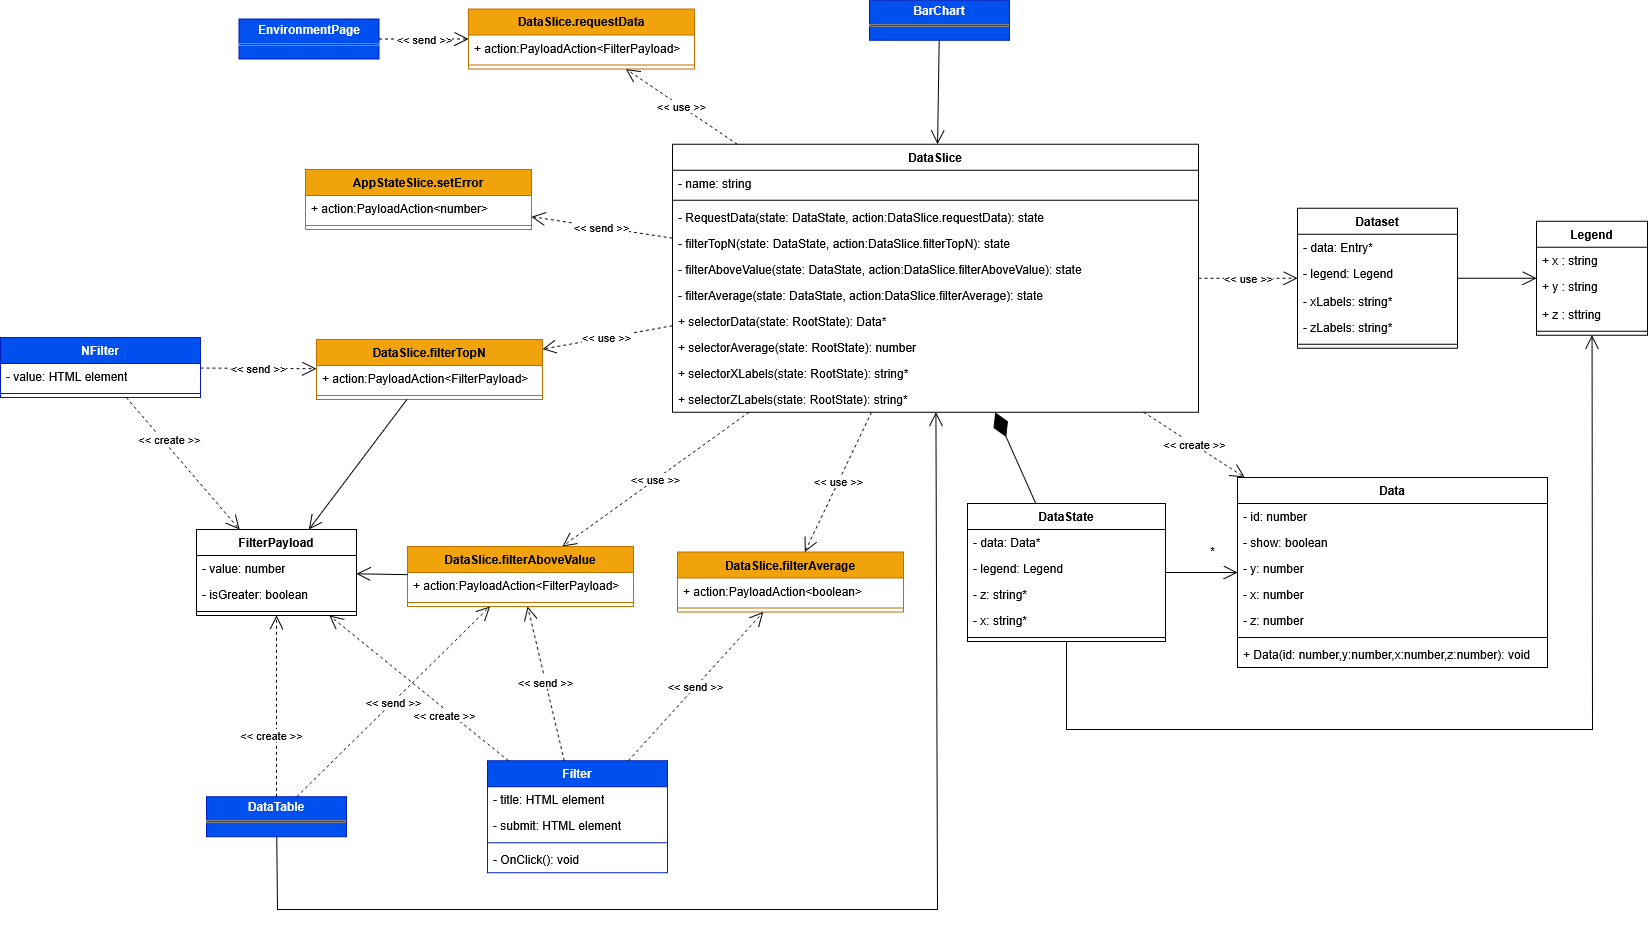
\includegraphics[scale=0.3]{template/images/uml_front/logic/dataslice.png}
    \caption{DataSlice}
\end{figure}
\textbf{Descrizione del diagramma:}\\
Questo diagramma include tutti i componenti utili per recuperare e filtrare i dati provenienti dal server.
\begin{itemize}
    \item \textbf{DataSlice:}
          \begin{itemize}
              \item \textbf{Dipendenze:}
                    \begin{itemize}
                        \item DataState (composizione): gestisce la creazione e la distruzione dell'istanza
                              di DataState, che non è condivisa con altri componenti;
                        \item RawData (dipendenza semplice <<use>>): rappresenta una singola entry del
                              dataset;
                        \item Data (dipendenza semplice <<create>>): responsabile della creazione dei singoli
                              oggetti Data che verranno inseriti nella lista di dati di DataState;
                        \item DataSlice.requestData (dipendenza semplice <<use>>): cattura un'istanza di
                              DataSlice.requestData e il reducer manda una richiesta al server per prendere i
                              dati del dataset selezionato utilizzando il payload;
                        \item DataSlice.filterTopN (dipendenza semplice <<use>>): cattura un'istanza di
                              DataSlice.filterTopN e il reducer applica un filtro sui primi N valori più alti
                              o più bassi, basandosi sui parametri di FilterPayload;
                        \item DataSlice.filterAverage (dipendenza semplice <<use>>): cattura un'istanza di
                              DataSlice.filterAverage e il reducer applica un filtro sui valori maggiori o
                              minori rispetto alla media globale, basandosi sui parametri di FilterPayload;
                        \item DataSlice.filterAboveValue (dipendenza semplice <<use>>): cattura un'istanza di
                              DataSlice.filterAboveValue e il reducer applica un filtro sui valori maggiori o
                              minori rispetto al valore della barra del grafico 3D selezionata, basandosi sui
                              parametri di FilterPayload;
                        \item AppStateSlice.setError (dipendenza semplice <<send>>): crea ed emette
                              un'istanza dell'azione AppStateSlice.setError.
                    \end{itemize}
              \item \textbf{Interazioni:}
                    \begin{itemize}
                        \item DataState: viene modificato in base alle action catturate dal reducer della
                              slice.
                    \end{itemize}
              \item \textbf{Action catturate:}
                    \begin{itemize}
                        \item DataSlice.filterTopN;
                        \item DataSlice.filterAverage;
                        \item DataSlice.filterAboveValue.
                    \end{itemize}
              \item \textbf{Action emesse:}
                    \begin{itemize}
                        \item AppStateSlice.setError.
                    \end{itemize}
          \end{itemize}

    \item \textbf{DataState:}
          \begin{itemize}
              \item \textbf{Dipendenze:}
                    \begin{itemize}
                        \item Data (associazione): contiene la lista dei dati del dataset.
                        \item Legend (associazione): contiene la legenda del dataset.
                    \end{itemize}
          \end{itemize}

    \item \textbf{Dataset:}
          \begin{itemize}
              \item \textbf{Dipendenze:}
                    \begin{itemize}
                        \item Legend (associazione): contiene la legenda del dataset.
                    \end{itemize}
          \end{itemize}

    \item \textbf{NFilter:}
          \begin{itemize}
              \item \textbf{Dipendenze:}
                    \begin{itemize}
                        \item DataSlice.filterTopN (dipendenza semplice <<send>>): crea ed emette un'istanza
                              dell'azione DataSlice.filterTopN;
                        \item FilterPayload (dipendenza semplice <<create>>): responsabile della creazione
                              dei payload di tipo FilterPayload che verranno poi utilizzati per applicare un
                              filtro nel modo corretto.
                    \end{itemize}
              \item \textbf{Action emesse:}
                    \begin{itemize}
                        \item DataSlice.filterTopN;
                    \end{itemize}
          \end{itemize}

    \item \textbf{Filter:}
          \begin{itemize}
              \item \textbf{Dipendenze:}
                    \begin{itemize}
                        \item DataSlice.filterAverage (dipendenza semplice <<send>>): crea ed emette
                              un'istanza dell'azione DataSlice.filterAverage;
                        \item DataSlice.filterAboveValue (dipendenza semplice <<send>>): crea ed emette
                              un'istanza dell'azione DataSlice.filterAboveValue;
                        \item FilterPayload (dipendenza semplice <<create>>): responsabile della creazione
                              dei payload di tipo FilterPayload che verranno poi utilizzati per applicare un
                              filtro nel modo corretto.
                    \end{itemize}
              \item \textbf{Action emesse:}
                    \begin{itemize}
                        \item DataSlice.filterAverage;
                        \item DataSlice.filterAboveValue.
                    \end{itemize}
          \end{itemize}

    \item \textbf{DataTable:}
          \begin{itemize}
              \item \textbf{Dipendenze:}
                    \begin{itemize}
                        \item DataSlice (associazione): contiene implicitamente un'istanza di DataSlice;
                        \item DataSlice.filterAboveValue (dipendenza semplice <<send>>): crea ed emette
                              un'istanza dell'azione DataSlice.DataSlice;
                        \item FilterPayload (dipendenza semplice <<create>>): responsabile della creazione
                              dei payload di tipo FilterPayload che verranno poi utilizzati per applicare un
                              filtro nel modo corretto.
                    \end{itemize}
              \item \textbf{Interazioni:}
                    \begin{itemize}
                        \item DataSlice: vengono utilizzati i metodi selectorData,selectorXLabels e
                              selectorZLabel per reperire la lista dei dati e delle etichette.
                    \end{itemize}
              \item \textbf{Action emesse:}
                    \begin{itemize}
                        \item DataSlice.filterAboveValue.
                    \end{itemize}
          \end{itemize}

    \item \textbf{BarChart:}
          \begin{itemize}
              \item \textbf{Dipendenze:}
                    \begin{itemize}
                        \item DataSlice (associazione): contiene implicitamente un'istanza di DataSlice.
                    \end{itemize}
              \item \textbf{Interazioni:}
                    \begin{itemize}
                        \item DataSlice: vengono utilizzati i metodi selectorData,selectorXLabels e
                              selectorZLabel per reperire la lista dei dati e delle etichette.
                    \end{itemize}
          \end{itemize}

    \item \textbf{EnvironmentPage:}
          \begin{itemize}
              \item \textbf{Dipendenze:}
                    \begin{itemize}
                        \item DataSlice.requestData (dipendenza semplice <<send>>): crea ed emette un'istanza
                              dell'azione DataSlice.requestData.
                    \end{itemize}
              \item \textbf{Action emesse:}
                    \begin{itemize}
                        \item DataSlice.requestData.
                    \end{itemize}
          \end{itemize}
\end{itemize}

\pagebreak

\paragraph{DataSourceSlice}
\begin{figure}[h!] \centering
    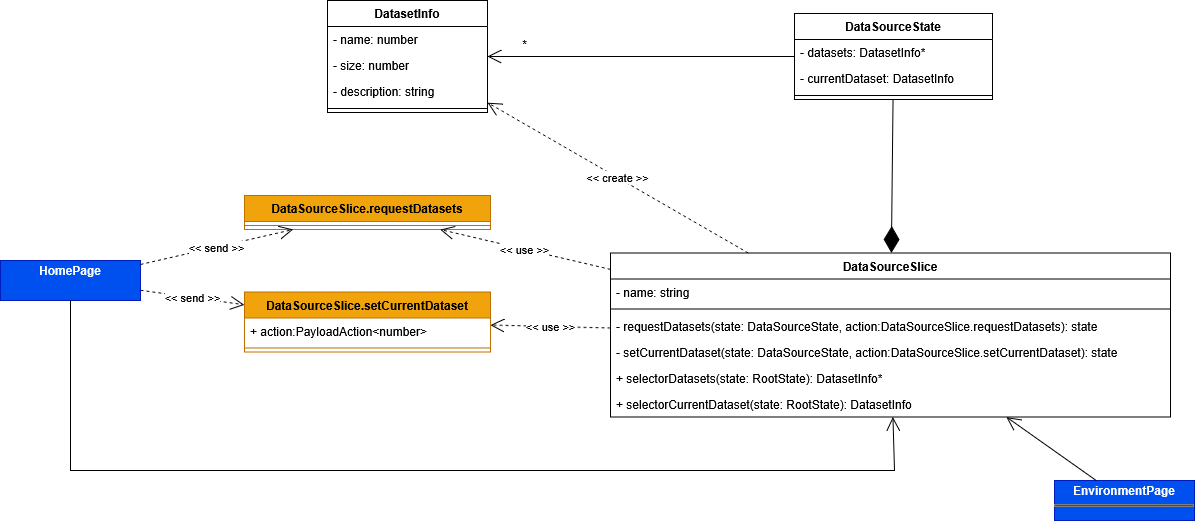
\includegraphics[scale=0.35]{template/images/uml_front/logic/datasourceslice.png}
    \caption{DataSourceSlice}
\end{figure}
\textbf{Descrizione del diagramma:}\\
Questo diagramma illustra i componenti per recuperare le informazioni chiave dai dataset proposti.
\begin{itemize}
    \item \textbf{DataSourceSlice:}
          \begin{itemize}
              \item \textbf{Dipendenze:}
                    \begin{itemize}
                        \item DataSourceState (composizione): gestisce la creazione e la distruzione
                              dell'istanza di DataSourceState, che non è condivisa con altri componenti;
                        \item DatasetInfo (dipendenza semplice <<create>>): responsabile della creazione dei
                              singoli oggetti DatasetInfo che verranno inseriti nella lista di dataset di
                              DataSourceState;
                        \item DataSourceSlice.requestData (dipendenza semplice <<use>>): cattura un'istanza
                              di DataSourceSlice.requestData e il reducer manda una richiesta al server per
                              prendere la lista dei dataset e le loro principali informazioni;
                        \item DataSourceSlice.setCurrentDataset (dipendenza semplice <<use>>): cattura
                              un'istanza di DataSourceSlice.setCurrentDataset e il reducer ne utilizza il
                              payload per aggiornare il dataset selezionato dall'utente.
                    \end{itemize}
              \item \textbf{Interazioni:}
                    \begin{itemize}
                        \item DataSourceState: viene modificato in base alle action catturate dal reducer
                              della slice.
                    \end{itemize}
              \item \textbf{Action catturate:}
                    \begin{itemize}
                        \item DataSourceSlice.setCurrentDataset;
                        \item DataSourceSlice.setCurrentDataset.
                    \end{itemize}
          \end{itemize}

    \item \textbf{DataSourceState:}
          \begin{itemize}
              \item \textbf{Dipendenze:}
                    \begin{itemize}
                        \item DatasetInfo (associazione): contiene la lista dei dataset proposti, con le loro
                              informazioni, e quello corrente.
                    \end{itemize}
          \end{itemize}

    \item \textbf{HomePage:}
          \begin{itemize}
              \item \textbf{Dipendenze:}
                    \begin{itemize}
                        \item DataSourceSlice (associazione): contiene implicitamente un'istanza di
                              DataSourceSlice;
                        \item DataLabelSlice.requestData (dipendenza semplice <<send>>): crea ed emette
                              un'istanza dell'azione DataLabelSlice.requestData;
                        \item DataLabelSlice.setCurrentDataset (dipendenza semplice <<send>>): crea ed emette
                              un'istanza dell'azione DataLabelSlice.setCurrentDataset.
                    \end{itemize}
              \item \textbf{Interazioni:}
                    \begin{itemize}
                        \item DataSourceSlice: viene utilizzato il metodo selectorDatasets per reperire la
                              lista dei dataset.
                    \end{itemize}
              \item \textbf{Action emesse:}
                    \begin{itemize}
                        \item DataLabelSlice.requestData;
                        \item DataLabelSlice.setCurrentDataset.
                    \end{itemize}
          \end{itemize}

    \item \textbf{EnvironmentPage:}
          \begin{itemize}
              \item \textbf{Dipendenze:}
                    \begin{itemize}
                        \item DataSourceSlice (associazione): contiene implicitamente un'istanza di
                              DataSourceSlice.
                    \end{itemize}
              \item \textbf{Interazioni:}
                    \begin{itemize}
                        \item DataSourceSlice: viene utilizzato il metodo selectorCurrentDataset per reperire
                              il dataset selezionato dall'utente e le sue informazioni.
                    \end{itemize}
          \end{itemize}
\end{itemize}

\paragraph{AppStateSlice}
\begin{figure}[h!] \centering
    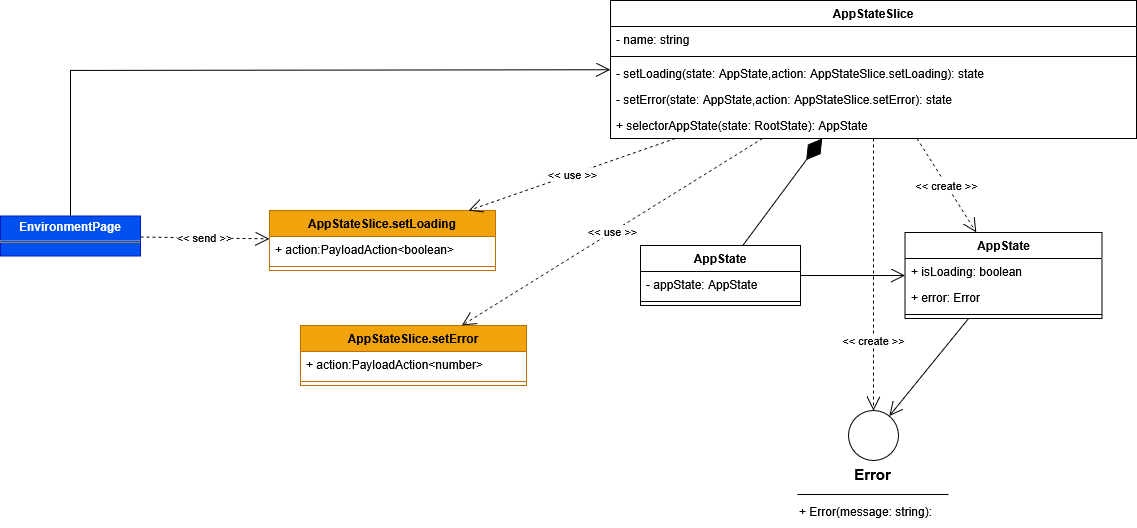
\includegraphics[scale=0.4]{template/images/uml_front/logic/appstateslice.png}
    \caption{AppStateSlice}
\end{figure}
\textbf{Descrizione del diagramma:}\\
Questo diagramma mostra i componenti per la gestione dello stato dell'applicazione.
\begin{itemize}
    \item \textbf{AppStateSlice:}
          \begin{itemize}
              \item \textbf{Dipendenze:}
                    \begin{itemize}
                        \item AppState (composizione): gestisce la creazione e la distruzione dell'istanza di
                              AppState, che non è condivisa con altri componenti;
                        \item AppState (dipendenza semplice <<create>>): responsabile della costruzione dell'
                              oggetto AppState inserire all'interno dell AppState;
                        \item AppStateSlice.setLoading (dipendenza semplice <<use>>): cattura un'istanza di
                              AppStateSlice.setLoading e il reducer aggiorna lo stato di caricamento
                              dell'applicazione utilizzando il payload;
                        \item AppStateSlice.setError (dipendenza semplice <<use>>): cattura un'istanza di
                              AppStateSlice.setError e il reducer aggiorna lo stato di errore
                              dell'applicazione ne utilizza il payload.
                    \end{itemize}
              \item \textbf{Interazioni:}
                    \begin{itemize}
                        \item DataSourceState: viene modificato in base alle action catturate dal reducer
                              della slice.
                    \end{itemize}
              \item \textbf{Action catturate:}
                    \begin{itemize}
                        \item AppStateSlice.setLoading;
                        \item AppStateSlice.setError.
                    \end{itemize}
          \end{itemize}

    \item \textbf{AppState:}
          \begin{itemize}
              \item \textbf{Dipendenze:}
                    \begin{itemize}
                        \item AppState (associazione): contiene l'oggetto che rappresenta lo stato
                              dell'applicazione.
                    \end{itemize}
          \end{itemize}

    \item \textbf{EnvironmentPage:}
          \begin{itemize}
              \item \textbf{Dipendenze:}
                    \begin{itemize}
                        \item AppStateSlice (associazione): contiene implicitamente un'istanza di
                              AppStateSlice;
                        \item AppStateSlice.setLoading (dipendenza semplice <<send>>): crea ed emette
                              un'istanza dell'azione AppStateSlice.setLoading.
                    \end{itemize}
              \item \textbf{Interazioni:}
                    \begin{itemize}
                        \item AppStateSlice: viene utilizzato il metodo selectorAppState per reperire lo
                              stato dell'applicazione.
                    \end{itemize}
              \item \textbf{Action emesse:}
                    \begin{itemize}
                        \item AppStateSlice.setLoading.
                    \end{itemize}
          \end{itemize}
\end{itemize}

\subparagraph{Error}
\begin{center}
    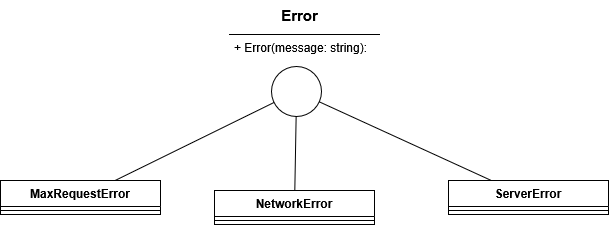
\includegraphics[scale=0.45]{template/images/uml_front/logic/error.png}
    \captionof{figure}{Error}
\end{center}
\textbf{Descrizione del diagramma:}\\
Questo diagramma mostra tutte le classi di errore.
\begin{itemize}
    \item \textbf{MaxRequestError:}
          \begin{itemize}
              \item \textbf{Dipendenze:}
                    \begin{itemize}
                        \item Error (implementazione): implementa una classe Error personalizzata, derivata
                              da una superclasse Error esistente, che include un messaggio specifico per gli
                              errori dovuti al superamento del limite di richieste.
                    \end{itemize}
          \end{itemize}

    \item \textbf{NetworkError:}
          \begin{itemize}
              \item \textbf{Dipendenze:}
                    \begin{itemize}
                        \item Error (implementazione): implementa una classe Error personalizzata, derivata
                              da una superclasse Error esistente, che include un messaggio specifico per gli
                              errori di rete non specifici.
                    \end{itemize}
          \end{itemize}

    \item \textbf{ServerError:}
          \begin{itemize}
              \item \textbf{Dipendenze:}
                    \begin{itemize}
                        \item Error (implementazione): implementa una classe Error personalizzata, derivata
                              da una superclasse Error esistente, che include un messaggio specifico per gli
                              errori di connessione non riuscita al server.
                    \end{itemize}
          \end{itemize}
\end{itemize}

\pagebreak

\paragraph{FilterOptionSlice}
\begin{figure}[h!] \centering
    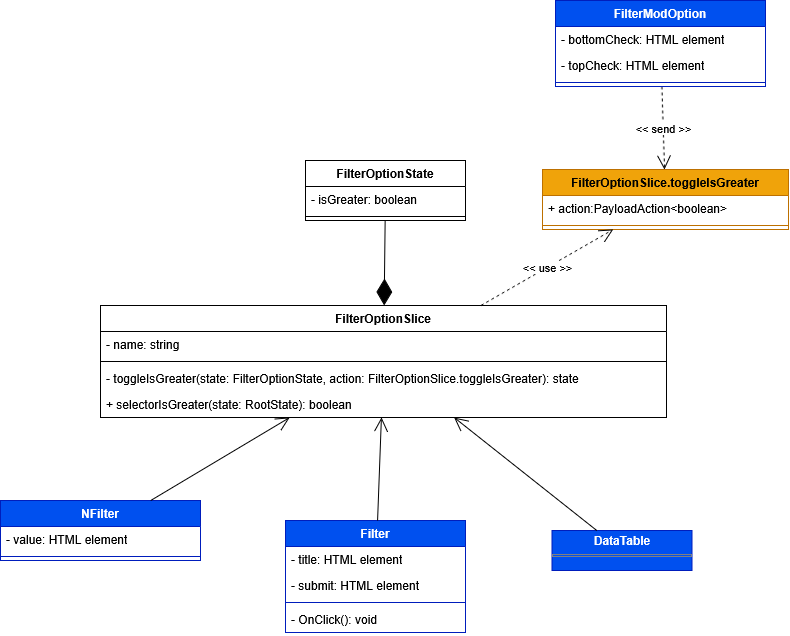
\includegraphics[scale=0.35]{template/images/uml_front/logic/filteroptionslice.png}
    \caption{FilterOptionSlice}
\end{figure}
\textbf{Descrizione del diagramma:}\\
Questo diagramma mostra i componenti per aggiornare e condividere le opzioni di filtraggio.
\begin{itemize}
    \item \textbf{FilterOptionSlice:}
          \begin{itemize}
              \item \textbf{Dipendenze:}
                    \begin{itemize}
                        \item FilterOptionState (composizione): gestisce la creazione e la distruzione
                              dell'istanza di FilterOptionState, che non è condivisa con altri componenti;
                        \item FilterOptionSlice.toggleIsGreater (dipendenza semplice <<use>>): cattura
                              un'istanza di FilterOptionSlice.toggleIsGreater e il reducer imposta il tipo di
                              filtraggio da effettuare utilizzando il payload.
                    \end{itemize}
              \item \textbf{Interazioni:}
                    \begin{itemize}
                        \item FilterOptionState: viene modificato in base alle action catturate dal reducer
                              della slice.
                    \end{itemize}
              \item \textbf{Action catturate:}
                    \begin{itemize}
                        \item FilterOptionSlice.toggleIsGreater.
                    \end{itemize}
          \end{itemize}

    \item \textbf{NFilter:}
          \begin{itemize}
              \item \textbf{Dipendenze:}
                    \begin{itemize}
                        \item FilterOptionSlice (associazione): contiene implicitamente un'istanza di
                              FilterOptionSlice.
                    \end{itemize}
              \item \textbf{Interazioni:}
                    \begin{itemize}
                        \item FilterOptionSlice: viene utilizzato il metodo selectorIsGreater per reperire le
                              opzioni per il filtraggio.
                    \end{itemize}
          \end{itemize}

    \item \textbf{Filter:}
          \begin{itemize}
              \item \textbf{Dipendenze:}
                    \begin{itemize}
                        \item FilterOptionSlice (associazione): contiene implicitamente un'istanza di
                              FilterOptionSlice.
                    \end{itemize}
              \item \textbf{Interazioni:}
                    \begin{itemize}
                        \item FilterOptionSlice: viene utilizzato il metodo selectorIsGreater per reperire le
                              opzioni per il filtraggio.
                    \end{itemize}
          \end{itemize}

    \item \textbf{DataTable:}
          \begin{itemize}
              \item \textbf{Dipendenze:}
                    \begin{itemize}
                        \item FilterOptionSlice (associazione): contiene implicitamente un'istanza di
                              FilterOptionSlice.
                    \end{itemize}
              \item \textbf{Interazioni:}
                    \begin{itemize}
                        \item FilterOptionSlice: viene utilizzato il metodo selectorIsGreater per reperire le
                              opzioni per il filtraggio.
                    \end{itemize}
          \end{itemize}

    \item \textbf{FilterModOption:}
          \begin{itemize}
              \item \textbf{Dipendenze:}
                    \begin{itemize}
                        \item FilterOptionSlice.toggleIsGreater (associazione semplice <<send>>): crea ed
                              emette un'istanza dell'azione FilterOption.toggleIsGreater.
                    \end{itemize}
              \item \textbf{Action emesse:}
                    \begin{itemize}
                        \item FilterOptionSlice.toggleIsGreater.
                    \end{itemize}
          \end{itemize}
\end{itemize}

\paragraph{ViewOptionSlice}
\begin{figure}[h!] \centering
    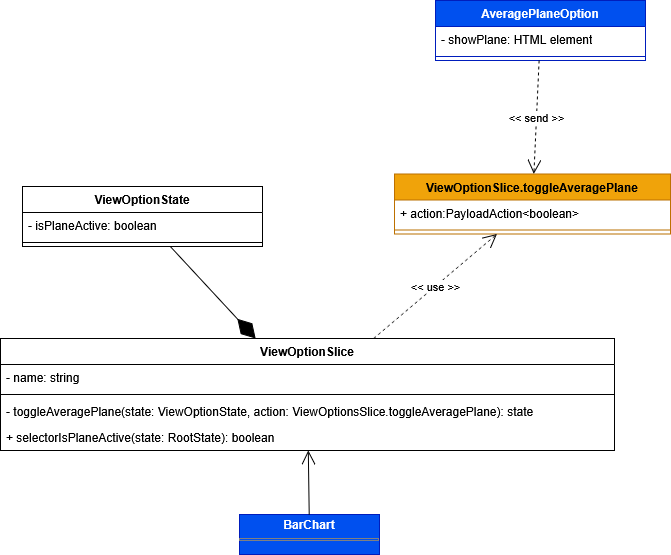
\includegraphics[scale=0.35]{template/images/uml_front/logic/viewoptionslice.png}
    \caption{FilterOptionSlice}
\end{figure}
\textbf{Descrizione del diagramma:}\\
Questo diagramma mostra i componenti per aggiornare e condividere le opzioni di visibilità del piano medio.
\begin{itemize}
    \item \textbf{FilterOptionSlice:}
          \begin{itemize}
              \item \textbf{Dipendenze:}
                    \begin{itemize}
                        \item ViewOptionState (composizione): gestisce la creazione e la distruzione
                              dell'istanza di FilterOptionState, che non è condivisa con altri componenti;
                        \item ViewOptionSlice.toggleAveragePlane (dipendenza semplice <<use>>): cattura
                              un'istanza di ViewOptionSlice.toggleAveragePlane e il reducer imposta la
                              visibilità del piano medio utilizzando il payload;
                    \end{itemize}
              \item \textbf{Interazioni:}
                    \begin{itemize}
                        \item ViewOptionState: viene modificato in base alle action catturate dal reducer
                              della slice.
                    \end{itemize}
              \item \textbf{Action catturate:}
                    \begin{itemize}
                        \item ViewOptionSlice.toggleAveragePlane;
                    \end{itemize}
          \end{itemize}

    \item \textbf{AveragePlaneOption:}
          \begin{itemize}
              \item \textbf{Dipendenze:}
                    \begin{itemize}
                        \item ViewOptionSlice.toggleAveragePlane (associazione semplice <<send>>): crea ed
                              emette un'istanza dell'azione ViewOptionSlice.toggleAveragePlane.
                    \end{itemize}
              \item \textbf{Action emesse:}
                    \begin{itemize}
                        \item ViewOptionSlice.toggleAveragePlane.
                    \end{itemize}
          \end{itemize}

    \item \textbf{BarChart:}
          \begin{itemize}
              \item \textbf{Dipendenze:}
                    \begin{itemize}
                        \item ViewOptionSlice (associazione): contiene implicitamente un'istanza di
                              ViewOptionSlice.
                    \end{itemize}
              \item \textbf{Interazioni:}
                    \begin{itemize}
                        \item ViewOptionSlice: viene utilizzato il metodo selectorIsPlaneActive per reperire
                              le opzioni di visibilità.
                    \end{itemize}
          \end{itemize}

\end{itemize}

\paragraph{RaycastHitSlice}
\begin{figure}[h!] \centering
    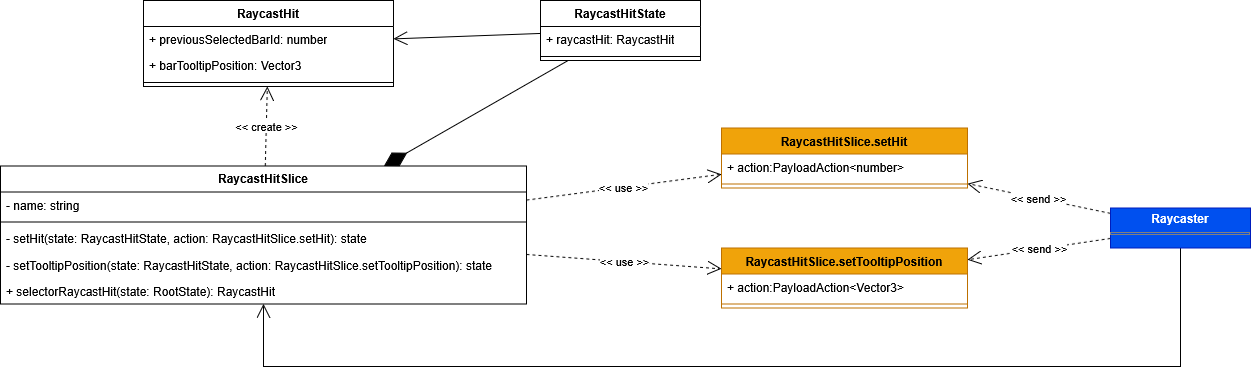
\includegraphics[scale=0.35]{template/images/uml_front/logic/raycastslice.png}
    \caption{RaycastHitSlice}
\end{figure}
\textbf{Descrizione del diagramma:}\\
Questo diagramma mostra i componenti per aggiornare e condividere le informazioni del raycast.
\begin{itemize}
    \item \textbf{RaycastHitSlice:}
          \begin{itemize}
              \item \textbf{Dipendenze:}
                    \begin{itemize}
                        \item RaycastHitState (composizione): gestisce la creazione e la distruzione
                              dell'istanza di RaycastHitState, che non è condivisa con altri componenti;
                        \item RaycastHit (dipendenza semplice <<create>>): responsabile della costruzione del
                              RaycastHit da inserire all'interno del RaycastHitState;
                        \item RaycastHitSlice.setHit (dipendenza semplice <<use>>): cattura un'istanza di
                              RaycastHitSlice.setHit e il reducer memorizza la barra del grafico cliccata
                              dall'utente utilizzando il payload;
                        \item RaycastHitSlice.setTooltipPosition (dipendenza semplice <<use>>): cattura
                              un'istanza di AppStateSlice.setError e il reducer aggiorna la posizione del
                              tooltip utilizzando il payload.
                    \end{itemize}
              \item \textbf{Interazioni:}
                    \begin{itemize}
                        \item DataSourceState: viene modificato in base alle action catturate dal reducer
                              della slice.
                    \end{itemize}
              \item \textbf{Action catturate:}
                    \begin{itemize}
                        \item RaycastHitSlice.setHit;
                        \item RaycastHitSlice.setTooltipPosition.
                    \end{itemize}
          \end{itemize}

    \item \textbf{RaycastHitState:}
          \begin{itemize}
              \item \textbf{Dipendenze:}
                    \begin{itemize}
                        \item RaycastHit (associazione): contiene l'oggetto che rappresenta il punto di
                              intersezione tra il cursore del mouse e una barra del grafico.
                    \end{itemize}
          \end{itemize}

    \item \textbf{Raycaster:}
          \begin{itemize}
              \item \textbf{Dipendenze:}
                    \begin{itemize}
                        \item RaycastHitSlice (associazione): contiene implicitamente un'istanza di
                              RaycastHitSlice;
                        \item RaycastHitSlice.setHit (dipendenza semplice <<send>>): crea ed emette
                              un'istanza dell'azione RaycastHitSlice.setHit;
                        \item RaycastHitSlice.setToolTipPosition (dipendenza semplice <<send>>): crea ed
                              emette un'istanza dell'azione RaycastHitSlice.setToolTipPosition.
                    \end{itemize}
              \item \textbf{Interazioni:}
                    \begin{itemize}
                        \item RaycastHitSlice: viene utilizzato il metodo selectorRaycastHit per reperire le
                              informazioni del raycast.
                    \end{itemize}
              \item \textbf{Action emesse:}
                    \begin{itemize}
                        \item RaycastHitSlice.setHit;
                        \item RaycastHitSlice.setToolTipPosition.
                    \end{itemize}
          \end{itemize}
\end{itemize}

\paragraph{Redux store}
\begin{figure}[h!] \centering
    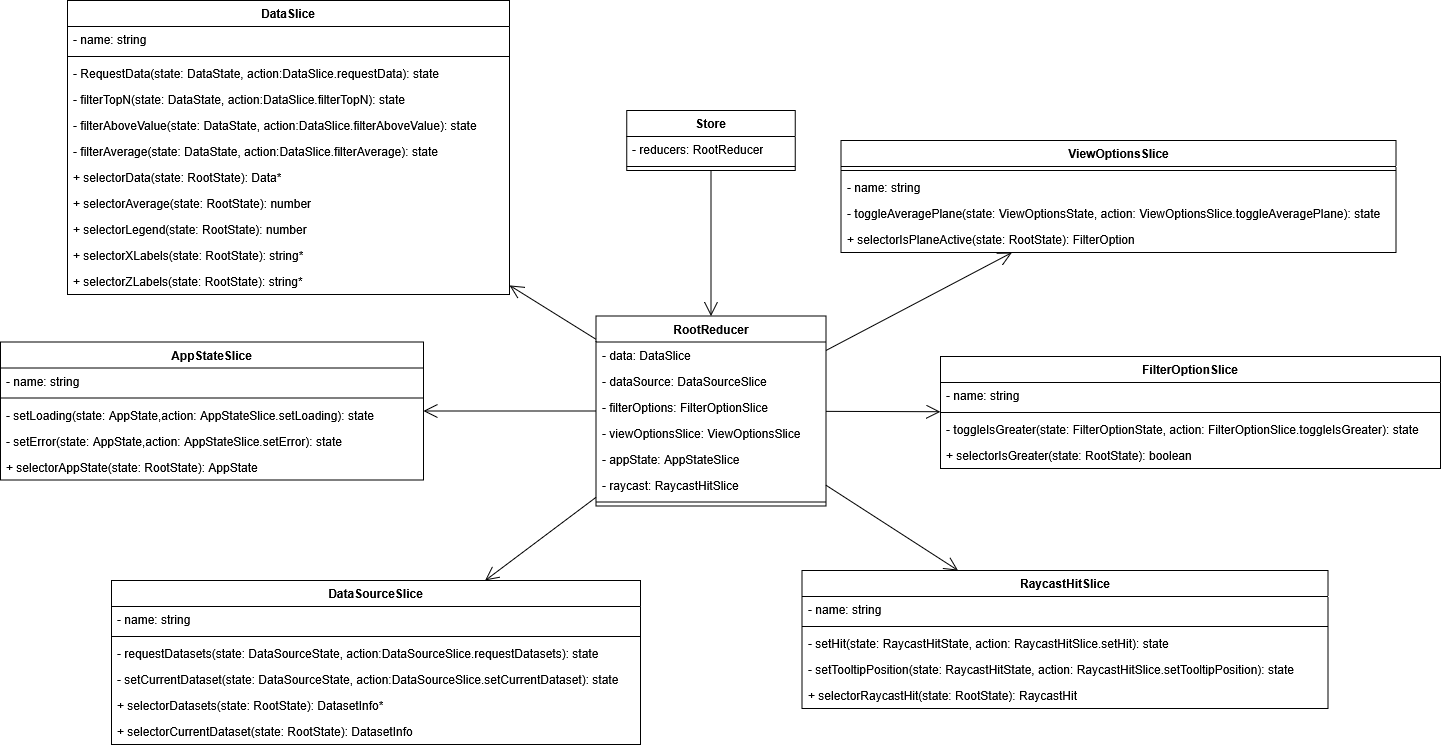
\includegraphics[scale=0.3]{template/images/uml_front/logic/store.png}
    \caption{Redux store}
\end{figure}
\textbf{Descrizione del diagramma:}\\
Questo diagramma mostra lo store e gli slice che compongono lo stato globale dell'applicazione.
\begin{itemize}
    \item \textbf{Store:}
          \begin{itemize}
              \item \textbf{Dipendenze:}
                    \begin{itemize}
                        \item RootReducer (associazione): possiede un attributo RootReducer che permette di
                              combinare più slice con cui lo store interagisce per modificare lo stato
                              globale dell'applicazione.
                    \end{itemize}
          \end{itemize}

    \item \textbf{RootReducer:}
          \begin{itemize}
              \item \textbf{Dipendenze:}
                    \begin{itemize}
                        \item DataSlice (associazione): possiede un attributo DataSlice per offrire allo
                              store l'accesso alla slice;
                        \item DataSourceSlice (associazione): possiede un attributo DataSourceSlice per
                              offrire allo store l'accesso alla slice;
                        \item FilterOptionSlice (associazione): possiede un attributo FilterOptionSlice per
                              offrire allo store l'accesso alla slice;
                        \item ViewOptionSlice (associazione): possiede un attributo ViewOptionSlice per
                              offrire allo store l'accesso alla slice;
                        \item AppStateSlice (associazione): possiede un attributo AppStateSlice per offrire
                              allo store l'accesso alla slice;
                        \item RaycastHitSlice (associazione): possiede un attributo RaycastHitSlice per
                              offrire allo store l'accesso alla slice.
                    \end{itemize}
          \end{itemize}
\end{itemize}

\paragraph{Pages}
\begin{figure}[h!] \centering
    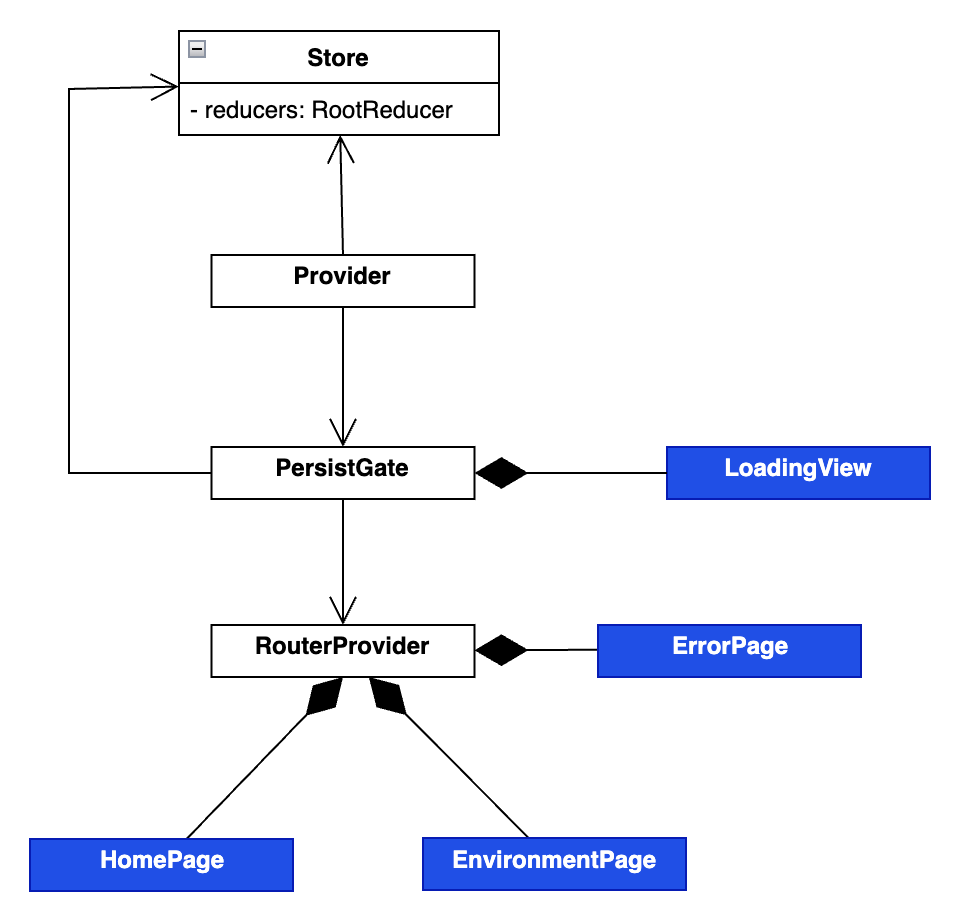
\includegraphics[scale=0.45]{template/images/uml_front/ui/pages.png}
    \caption{Pages}
\end{figure}
\textbf{Descrizione del diagramma:}
Questo diagramma mostra come sono organizzate le varie pagine dell'applicazione.
\begin{itemize}
    \item \textbf{Provider:}
          \begin{itemize}
              \item \textbf{Dipendenze:}
                    \begin{itemize}
                        \item Store (associazione): utile al Provider di Redux per consentire l'accesso allo
                              store (e quindi allo stato globale) a tutti i componenti nella gerarchia;
                        \item RouterProvider (associazione): componente React che gestisce le pagine
                              dell'applicazione e le loro relative rotte.
                    \end{itemize}
          \end{itemize}

    \item \textbf{RouterProvider:}
          \begin{itemize}
              \item \textbf{Dipendenze:}
                    \begin{itemize}
                        \item HomePage (composizione): componente React che offre all'utente l'interfaccia
                              per la scelta del dataset desiderato;
                        \item EnvironmentPage (composizione): componente React che fornisce l'interfaccia per
                              visualizzare un dataset in un ambiente 3D;
                        \item ErrorPage (composizione): componente React responsabile della visualizzazione e
                              della gestione degli errori generati dall'applicazione.
                    \end{itemize}
          \end{itemize}

    \item \textbf{HomePage:}
          \begin{itemize}
              \item \textbf{Dipendenze:}
                    \begin{itemize}
                        \item DatasetItem (composizione): componente React dedicato alla presentazione delle
                              informazioni chiave di un dataset
                        \item Footer (composizione): componente React dedicato alla visualizzazione del
                              footer dell'applicazione;
                    \end{itemize}
          \end{itemize}
\end{itemize}

\pagebreak

\paragraph{EnvironmentPage}
\begin{figure}[h!] \centering
    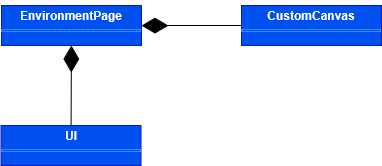
\includegraphics[scale=0.45]{template/images/uml_front/ui/envpage.png}
    \caption{EnvironmentPage}
\end{figure}
\textbf{Descrizione del diagramma:}
Questo diagramma presenta l'organizzazione degli elementi all'interno della pagina dedicata alla visualizzazione di un dataset in ambiente 3D.
\begin{itemize}
    \item \textbf{EnvironmentPage:}
          \begin{itemize}
              \item \textbf{Dipendenze:}
                    \begin{itemize}
                        \item UI (composizione): componente React che avvolge e gestisce l'intera UI
                              dell'applicazione;
                        \item CustomCanvas (composizione): componente React responsabile della
                              visualizzazione e del rendering dell'ambiente 3D.
                    \end{itemize}
          \end{itemize}
\end{itemize}

\paragraph{UI}
\begin{figure}[h!] \centering
    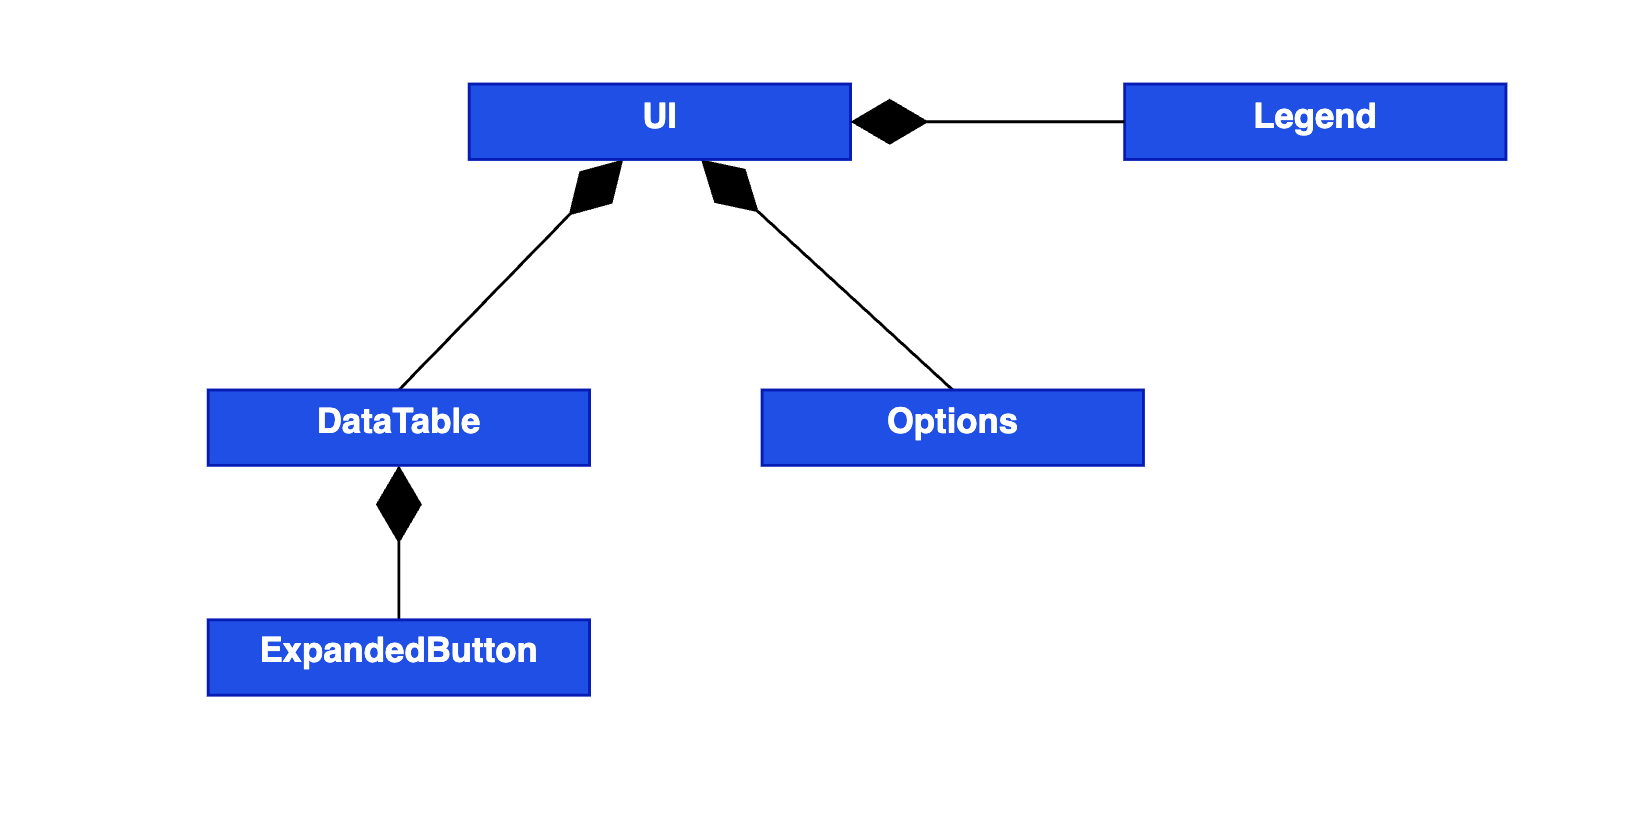
\includegraphics[scale=0.45]{template/images/uml_front/ui/ui.png}
    \caption{UI}
\end{figure}
\textbf{Descrizione del diagramma:}
Questo diagramma presenta la struttura e gli elementi che costituiscono la UI dell'applicazione.
\begin{itemize}
    \item \textbf{UI:}
          \begin{itemize}
              \item \textbf{Dipendenze:}
                    \begin{itemize}
                        \item Footer (composizione): componente React dedicato alla visualizzazione del
                              footer dell'applicazione;
                        \item DataTable (composizione): componente React dedicato alla presentazione di un
                              dataset in formato tabellare;
                        \item Options (composizione): componente React dedicato alla visualizzazione di
                              un form contenente le opzioni per filtrare i dati.
                    \end{itemize}
          \end{itemize}
\end{itemize}

\pagebreak

\paragraph{Options}
\begin{figure}[h!] \centering
    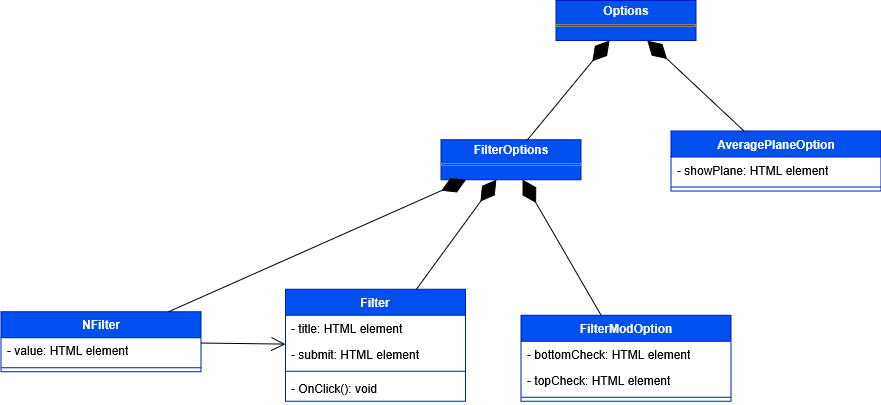
\includegraphics[scale=0.45]{template/images/uml_front/ui/options.png}
    \caption{Options}
\end{figure}
\textbf{Descrizione del diagramma:}
Questo diagramma evidenzia la struttura dei gruppi in cui sono suddivise le opzioni di filtraggio e visibilità del piano medio.
\begin{itemize}
    \item \textbf{Options:}
          \begin{itemize}
              \item \textbf{Dipendenze:}
                    \begin{itemize}
                        \item FilterOptions (composizione): componente React che raggruppa le opzioni di
                              filtraggio;
                        \item AveragePlaneOption (composizione): componente React che implementa un filtro
                              generico capace di filtrare valori superiori o inferiori rispetto a un dato
                              valore di riferimento;
                    \end{itemize}
          \end{itemize}

    \item \textbf{FilterOption:}
          \begin{itemize}
              \item \textbf{Dipendenze:}
                    \begin{itemize}
                        \item NFilter (composizione): componente React che offre la possibilità eseguire un
                              filtraggio sul dataset visualizzando solo i primi N valori più alti o più
                              bassi;
                        \item Filter (composizione): componente React che implementa un filtro generico
                              capace di eseguire un filtraggio visualizzando valori superiori o inferiori
                              rispetto a un dato valore di riferimento;
                        \item FilterModOption (composizione): componente React che visualizza un form per
                              permettere all'utente di scegliere se il filtro opererà su valori maggiori o
                              minori;
                    \end{itemize}
          \end{itemize}

    \item \textbf{NFilter:}
          \begin{itemize}
              \item \textbf{Dipendenze:}
                    \begin{itemize}
                        \item Filter (associazione): componente React che implementa un filtro generico
                              capace di filtrare valori superiori o inferiori rispetto a un dato valore di
                              riferimento. In questo caso, è stato esteso per includere un campo che permette
                              di specificare un valore N.
                    \end{itemize}
          \end{itemize}
\end{itemize}

\pagebreak

\paragraph{Custom canvas}
\begin{figure}[h!] \centering
    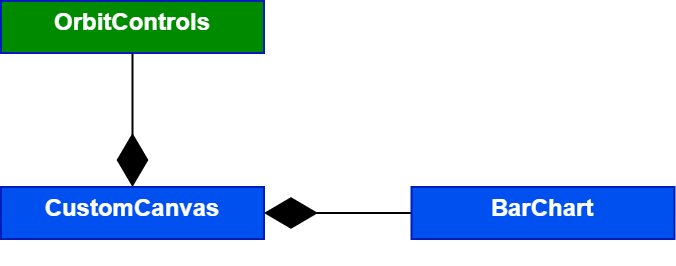
\includegraphics[scale=0.45]{template/images/uml_front/ui/customcanvas.png}
    \caption{Custom canvas}
\end{figure}
\textbf{Descrizione del diagramma:}
Questo diagramma presenta la struttura e gli elementi che costituiscono l'ambiente 3D.
\begin{itemize}
    \item \textbf{CustomCanvas:}
          \begin{itemize}
              \item \textbf{Dipendenze:}
                    \begin{itemize}
                        \item OrbitControls (composizione): componente React Three Fiber che abilita la
                              navigazione e la manipolazione della telecamera 3D utilizzando gli input del
                              mouse;
                        \item BarChart (composizione): componente React che racchiude e gestisce l'intera
                              struttura del grafico 3D.
                    \end{itemize}
          \end{itemize}
\end{itemize}

\paragraph{Bar chart}
\begin{figure}[h!] \centering
    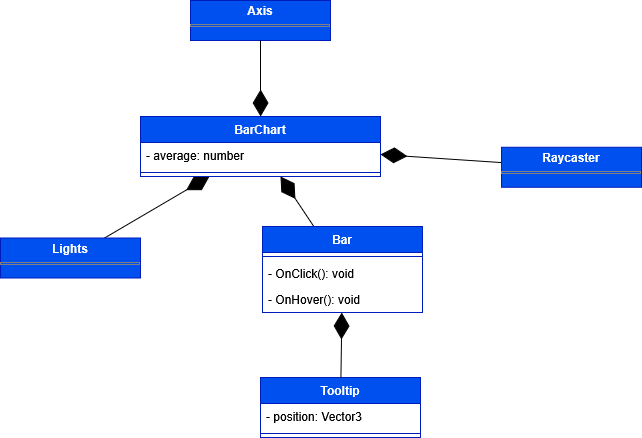
\includegraphics[scale=0.45]{template/images/uml_front/ui/barchart.png}
    \caption{Bar chart}
\end{figure}
\textbf{Descrizione del diagramma:}
Questo diagramma presenta gli elementi che costituiscono il grafico 3D.
\begin{itemize}
    \item \textbf{BarChart:}
          \begin{itemize}
              \item \textbf{Dipendenze:}
                    \begin{itemize}
                        \item Axis (composizione): componente React che contiene gli assi X, Y e Z del
                              grafico 3D;
                        \item AveragePlane (composizione): componente React che permette di visualizzare il
                              piano medio sul grafico 3D;
                        \item Lights (composizione): componente React per la gestione delle luci
                              nell'ambiente 3D;
                        \item Raycaster (composizione): componente React che implementa la logica per
                              determinare se e dove il cursore del mouse interseca una barra del grafico;
                        \item Bars (composizione): componente React dedicato al rendering degli elementi che
                              rappresentano le barre all'interno del grafico 3D.
                    \end{itemize}
          \end{itemize}

    \item \textbf{Bars:}
          \begin{itemize}
              \item \textbf{Dipendenze:}
                    \begin{itemize}
                        \item Tooltip (composizione): componente React per visualizzare un riquadro
                              informativo al passaggio del mouse sopra la barra del grafico.
                    \end{itemize}
          \end{itemize}
\end{itemize}

\paragraph{Axes}
\begin{figure}[h!] \centering
    
\includegraphics[scale=0.45]{template/images/uml_front/ui/axes.png}
    \caption{Axes}
\end{figure}
\textbf{Descrizione del diagramma:}
Questo diagramma presenta gli elementi che costituiscono ciascuno dei tre assi del grafico 3D.
\begin{itemize}
    \item \textbf{Axes:}
          \begin{itemize}
              \item \textbf{Dipendenze:}
                    \begin{itemize}
                        \item XAxis (composizione): componente React che rappresenta l'asse X del grafico 3D
                              con relative etichette;
                        \item YAxis (composizione): componente React che rappresenta l'asse Y del grafico 3D
                              con relative etichette;
                        \item ZAxis (composizione): componente React che rappresenta l'asse Z del grafico 3D
                              con relative etichette.
                    \end{itemize}
          \end{itemize}
\end{itemize}
\pagebreak

\subsection{Architettura backend}

\subsubsection{Descrizione generale} 
L’architettura del backend adotta lo stile modulare fornito da NestJS, con moduli principali che gestiscono le funzionalità chiave dell'applicazione e moduli di supporto che forniscono risorse necessari a quelli precedenti. I moduli principali sono organizzati secondo un approccio a layer, comprendente controller, servizi e repository.\\
Il ruolo principale del backend è quello di fungere da mediatore tra diverse fonti di dati esterne (principalmente API REST), aggregando e trasformando le informazioni ricevute in un formato uniforme e coerente. I dati vengono quindi resi disponibili tramite endpoint REST standardizzati. Le sorgenti dati sono gestite da componenti chiamati \textit{fetcher}, ciascuno progettato per interagire con un'API specifica. Tutti i \textit{fetcher} seguono la stessa interfaccia, il che rende facile aggiungere nuove fonti di dati in futuro.

\subsubsection{Diagramma delle classi}
\begin{figure}[H]
    \begin{center}
        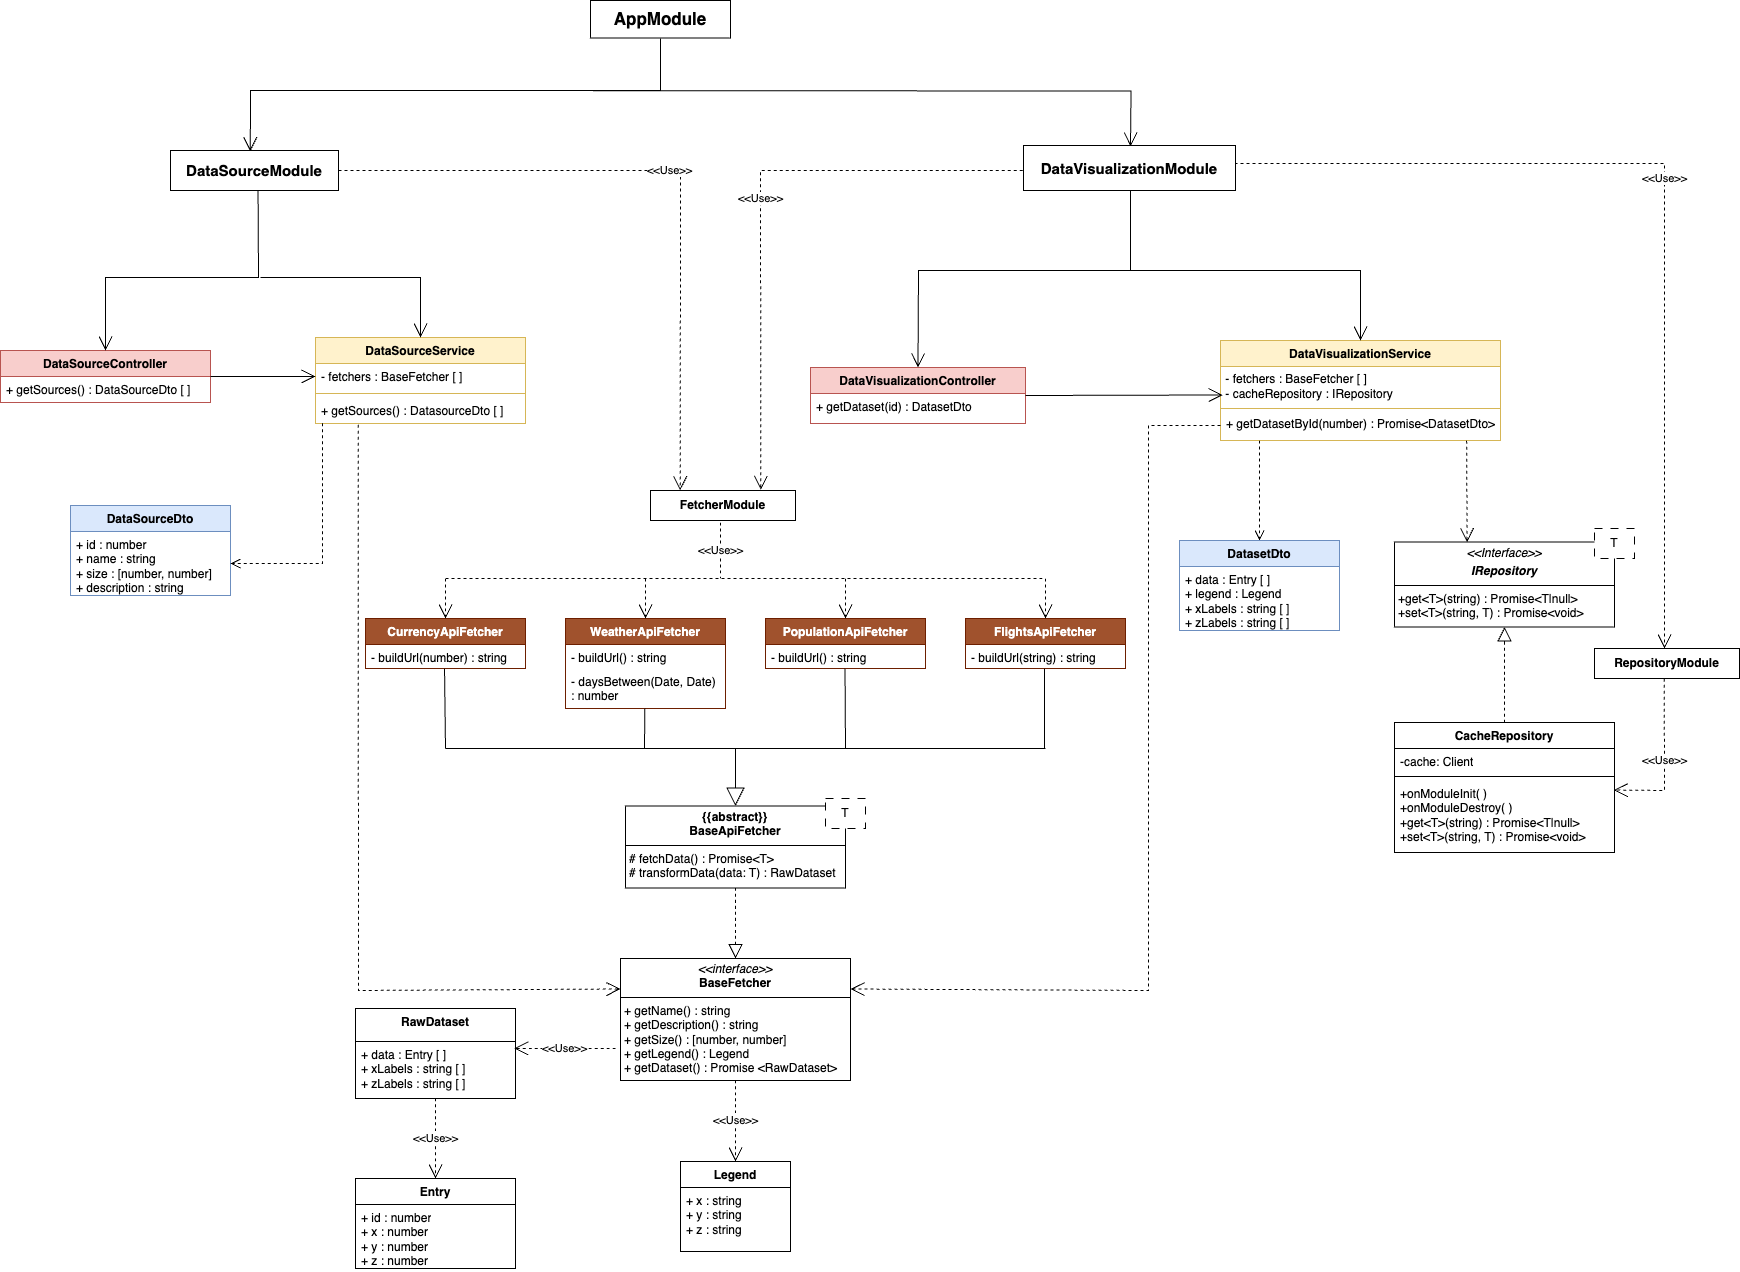
\includegraphics[scale = 0.29]{template/images/uml_back/BackendUML.png}
        \caption{Diagramma delle classi del backend}
    \end{center}     
    
\end{figure}

\subsubsection{Moduli}

L'architettura del sistema è suddivisa in moduli specializzati, ognuno dei quali gestisce una funzionalità o un'area logica specifica dell'applicazione. Questa organizzazione facilita l’indipendenza tra componenti, promuove il riuso del codice e permette di mantenere alta la qualità progettuale anche in presenza di modifiche o estensioni future.
Ogni modulo interagisce con il resto del sistema attraverso interfacce ben definite. Questo approccio, ispirato alla programmazione modulare.\\
In NestJS, ogni modulo è una classe annotata con un decoratore \texttt{@Module()} che organizza logicamente i componenti dell’applicazione, come controller e servizi. L’integrazione tra moduli avviene tramite il sistema di imports ed exports, che consente di condividere funzionalità in modo esplicito e controllato.

\paragraph{AppModule}

\begin{figure}[H] 
    \centering
    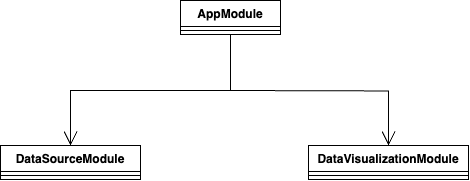
\includegraphics[scale = 0.5]{template/images/uml_back/AppModule.png}
    \caption{AppModule}
\end{figure}

L'AppModule rappresenta il punto di ingresso dell'applicazione e la sua funzione principale è quella di gestire e configurare i moduli principali. Questo modulo carica e configura i moduli \texttt{DataSourceModule} e \texttt{DataVisualizationModule}.

\paragraph{Moduli principali}
I moduli principali contengono la logica fondamentale dell'applicazione e sono responsabili della gestione e visualizzazione dei dati. I principali moduli dell'applicazione sono i seguenti:

\subparagraph{DataSourceModule}: 

\begin{figure}[H] 
    \centering
    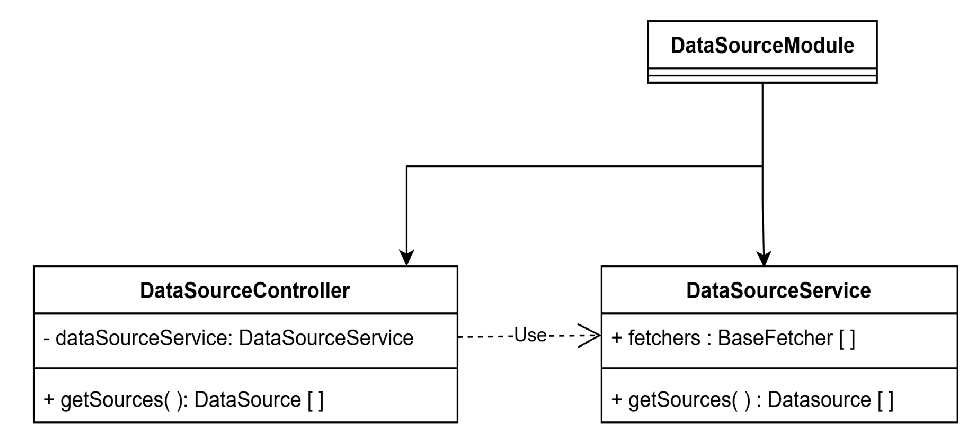
\includegraphics[scale = 0.55]{template/images/uml_back/DataSourceModule.png}
    \caption{DataSourceModule}
\end{figure}

Il \texttt{DataSourceModule} è responsabile della gestione delle metainformazioni relative alle fonti di dati disponibili nel sistema. Questo modulo incapsula la logica necessaria per raccogliere, organizzare e fornire informazioni descrittive sui dataset che l'applicazione può visualizzare.\\

\textbf{Responsabilità:}
\begin{itemize}
    \item Fornire un catalogo completo delle fonti dati disponibili;
    \item Recuperare metadati descrittivi per ciascuna fonte (nome, dimensione, descrizione);
    \item Esporre queste informazioni attraverso endpoint REST;
    \item Organizzare i metadati in strutture DTO coerenti per il consumo da parte del frontend.
\end{itemize}

\textbf{Componenti:}
\begin{itemize}
    \item \texttt{DataSourceController}: espone l'endpoint HTTP \texttt{GET /data-source} che restituisce la lista completa delle fonti dati disponibili. Gestisce le richieste in arrivo, le instrada al servizio appropriato e serializza le risposte.
    
    \item \texttt{DataSourceService}: implementa la logica di business per la raccolta dei metadati. Si interfaccia con i \texttt{fetcher} disponibili tramite l'interfaccia \texttt{BaseFetcher}, interrogando ciascuno per ottenere le informazioni descrittive necessarie. Questo servizio è responsabile della trasformazione dei dati grezzi in oggetti \texttt{DataSourceDto} ben strutturati.
    
    \item \texttt{DataSourceDto}: definisce la struttura dei dati trasferiti dal backend al frontend. Include:
    \begin{itemize}
        \item \texttt{id}: identificatore univoco della fonte dati;
        \item \texttt{name}: nome descrittivo della fonte;
        \item \texttt{size}: dimensione del dataset;
        \item \texttt{description}: descrizione dettagliata del contenuto della fonte.
    \end{itemize}
\end{itemize}

\textbf{Dipendenze:}
\begin{itemize}
    \item \texttt{FetcherModule}: fornisce al \texttt{DataSourceService} l'accesso ai fetchers tramite il token di iniezione \texttt{FETCHERS}. Ciò consente al servizio di utilizzare i fetcher disponibili senza preoccuparsi delle loro implementazioni specifiche o della loro creazione e configurazione diretta;
    \item \texttt{BaseFetcher}: interfaccia che definisce il contratto che ogni fetcher deve rispettare, inclusi i metodi per ottenere metadati descrittivi come \texttt{getName()}, \texttt{getDescription()} e \texttt{getSize()}.
\end{itemize}

\subparagraph{DataVisualizationModule}:

\begin{figure}[H] 
    \centering
    \includegraphics[scale = 0.5]{template/images/uml_back/DataVisModule.png}
    \caption{DataVisualizationModule}
\end{figure}

Il \texttt{DataVisualizationModule} gestisce la logica di recupero e formattazione dei dataset per la visualizzazione.\\

\textbf{Responsabilità:}
\begin{itemize}
    \item Recuperare il dataset completo dal fonte selezionato dall'utente tramite un ID specifico;
    \item Communicare con il cache per velocizzare il caricamento dei dati già richiesti in precedenza;
    \item Esporre un endpoint REST standardizzato per l'accesso ai dataset formattati.
\end{itemize}

\textbf{Componenti:}
\begin{itemize}
    \item \texttt{DataVisualizationController}: espone l'endpoint HTTP \texttt{GET /data-visualization/:id} che accetta l'ID numerico di un dataset e restituisce il dataset completo corrispondente;
    \item \texttt{DataVisualizationService}: implementa la logica per il recupero del dataset richiesto. Il servizio verifica la validità dell'ID, controlla la disponibilità dei dati nella cache e, se necessario, utilizza il fetcher appropriato per ottenere i dati dalla fonte esterna;
    \item \texttt{DatasetDto}: definisce la struttura dei dati restituiti al frontend, composta da:
    \begin{itemize}
        \item \texttt{data}: array di \texttt{Entry}, dove ogni entry rappresenta un'unità di dati con il valore \texttt{y} associato agli indici di coordinate \texttt{x} e \texttt{z};
        \item \texttt{legend}: struttura di tipo \texttt{Legend}, contenente la legenda degli assi;
        \item \texttt{xLabels}: array di stringhe contenente le etichette per l'asse orizzontale.
        \item \texttt{zLabels}: array di stringhe contenente le etichette per l'asse verticale.
    \end{itemize}
\end{itemize}

\subparagraph{Dipendenze:}

\begin{itemize}
    \item \texttt{FetcherModule}: Fornisce accesso all'array di \texttt{BaseFetcher} attraverso il token di iniezione \texttt{FETCHERS}. Questo permette al \texttt{DataVisualizationService} di recuperare i dati da diverse fonti in modo modulare, senza dipendere dalle implementazioni specifiche dei fetchers;
    \item \texttt{RepositoryModule}: Esporta il \texttt{CacheRepository} come implementazione concreta dell'interfaccia \texttt{IRepository}. Questo consente al \texttt{DataVisualizationService} di interagire con la cache tramite un'interfaccia.
    \item \texttt{BaseFetcher}: Interfaccia che ogni fetcher implementa per fornire accesso standardizzato ai dati;
    \item \texttt{IRepository}: Interfaccia generica che fornisce un contratto per le operazioni di lettura e scrittura di dati;
    \begin{itemize}
        \item \texttt{get(key: string)}: recupera un valore
        \item \texttt{set(key: string, value: T)}: salva un valore.
    \end{itemize}
    \item \texttt{CacheRepository}: Classe che implementa \texttt{IRepository}, fornendo la logica concreta per la lettura e scrittura nella cache. Registrata e esportata dal \texttt{RepositoryModule}.
\end{itemize}


\paragraph{Moduli di supporto}
I moduli di supporto forniscono funzionalità tecniche o infrastrutturali necessarie al funzionamento dell’applicazione.
Essi vengono progettati per essere riutilizzabili, indipendenti e incapsulati. Vengono esportati verso i moduli principali che ne fanno uso.
In questo progetto includono il \texttt{FetcherModule} e il \texttt{RepositoryModule}, che offrono rispettivamente l'accesso ai dati esterni e la logica di persistenza tramite cache.


\subparagraph{FetcherModule}:

\begin{figure}[H] 
    \centering
    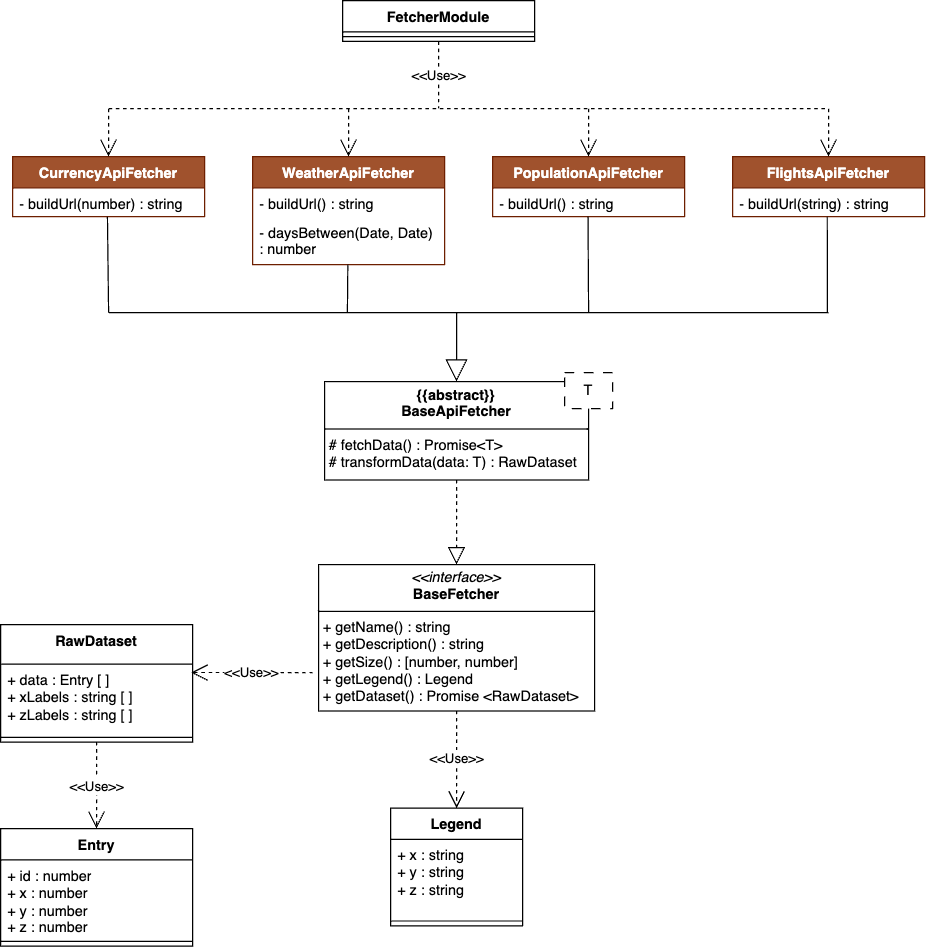
\includegraphics[scale = 0.5]{template/images/uml_back/FetcherModule.png}
    \caption{FetcherModule}
\end{figure}

Il \texttt{FetcherModule} incapsula tutti i componenti responsabili del recupero dei dati da fonti esterne, come API. Non contiene logica di business, ma espone un'interfaccia coerente per l’accesso ai dati, facilitando l’estensione e la manutenibilità del sistema.\\

\textbf{Responsabilità:}
\begin{itemize}
    \item Registrare e gestire i diversi \texttt{fetcher} che implementano l’interfaccia \texttt{BaseFetcher};
    \item Fornire un punto di accesso centralizzato e modulare alle fonti dati esterne.
\end{itemize}

\textbf{Struttura del modulo:}
\begin{itemize}
    \item \texttt{BaseFetcher}: interfaccia che definisce il contratto da rispettare per ogni \texttt{fetcher};
    \item \texttt{BaseApiFetcher}: classe astratta che offre una base comune per tutti i \texttt{fetcher} basati su API REST;
    \item \texttt{RawDataset}: struttura che rappresenta il formato iniziale dei dati raccolti, composto da una lista di entry e da etichette associate agli assi orizzontale e verticale;
    \item \texttt{Entry}: struttura che definisce un'unità di dati con il valore \texttt{y} associato agli indici di coordinate \texttt{x} e \texttt{z};
    \item \texttt{Legend}: struttura che definisce la legenda degli assi.
    
    La separazione tra \texttt{BaseFetcher} e \texttt{BaseApiFetcher} consente di favorire la riusabilità e la manutenzione del codice. Mentre \texttt{BaseFetcher} stabilisce un'interfaccia generica per qualsiasi sorgente dati, \texttt{BaseApiFetcher} si occupa della gestione specifica delle API REST, implementando i metodi \texttt{fetchData} e \texttt{transformData}, che sono propri dei fetcher per API. Questo approccio centralizza la logica comune legata alle API, evitando la duplicazione del codice.
    
\end{itemize}

\textbf{Fetcher concreti:}
\begin{itemize}
    \item \texttt{WeatherApiFetcher}: recupera informazioni sulla temperatura media oraria per alcune grandi città europee, dal 01/01/2025 al 31/03/2025;
    \item \texttt{PopulationApiFetcher}: ottiene dataset contenente la popolazione totale di alcuni paesi dal 1974 al 2023;
    \item \texttt{FlightsApiFetcher}: fornisce il numero di partenze aeree da alcuni aeroporti internazionali nelle diverse fasce orarie in una giornata;
    \item \texttt{CurrencyApiFetcher}: restituisce tassi di cambio rispetto all'Euro campionati all'inizio di ogni anno dal 2005 al 2025.
\end{itemize}

\textbf{Integrazione con altri moduli:} \\
Il \texttt{FetcherModule} esporta il provider \texttt{FETCHERS}, che aggrega le istanze concrete dei \texttt{fetcher}. Questo consente agli altri moduli dell’applicazione di iniettarli facilmente, seguendo i principi dell’inversione delle dipendenze.

\subparagraph{RepositoryModule}:

\begin{figure}[H] 
    \centering
    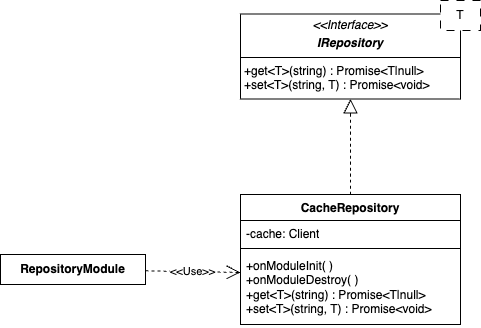
\includegraphics[scale = 0.5]{template/images/uml_back/RepositoryModule.png}
    \caption{RepositoryModule}
\end{figure}

Il \texttt{RepositoryModule} raggruppa i provider e i componenti che gestiscono la logica di persistenza dei dati, come il \texttt{CacheRepository}. Questo modulo fornisce un'interfaccia coerente per la gestione della cache ed è responsabile della persistenza temporanea dei dati. Utilizza \texttt{Memcached} tramite la libreria client \texttt{memjs}, per ottimizzare le performance dell'applicazione.

\textbf{Responsabilità:}
\begin{itemize}
    \item Fornire un meccanismo centrale per l’accesso ai dati temporanei;
    \item Isolare l’implementazione della cache dai servizi applicativi, attraverso l’uso di un’interfaccia.
\end{itemize}

\textbf{Struttura del modulo:}
\begin{itemize}
    \item \texttt{IRepository<T>}: interfaccia generica che definisce le operazioni base di salvataggio e lettura;
    \item \texttt{CacheRepository}: implementazione concreta che gestisce la connessione a Memcached e si occupa della serializzazione (conversione in stringa JSON) e deserializzazione dei dati per la loro corretta memorizzazione e recupero.
\end{itemize}

\textbf{Funzionalità del CacheRepository:}
\begin{itemize}
    \item Si connette al server Memcached all’avvio del modulo (\texttt{onModuleInit});
    \item Chiude la connessione in fase di distruzione del modulo (\texttt{onModuleDestroy});
    \item Metodo \texttt{get(key: string)}: recupera e deserializza il valore associato alla chiave specificata;
    \item Metodo \texttt{set(key: string, value: T)}: serializza e salva un valore con una chiave;
    \item Gestione robusta degli errori: i fallimenti di cache non interrompono il flusso del programma.
\end{itemize}

\textbf{Integrazione con altri moduli:} \\
Il modulo esporta la classe concreta \texttt{CacheRepository} come provider associato all'interfaccia \texttt{IRepository}. In questo modo, il \texttt{DataVisualizationService} dipende dall'interfaccia e mantiene un basso accoppiamento. \texttt{CacheRepository} viene creata e iniettata dal sistema di Dependency Injection.


\subsection{Pattern architetturale e Design pattern}

\subsubsection{Architettura Modulare (Modular Architecture)}
L’architettura del backend è progettata seguendo un approccio modulare, in cui ogni modulo rappresenta un'unità funzionale autonoma. Ciò consente di isolare le responsabilità, facilitando la manutenibilità e l'estensibilità del sistema. Ogni modulo è progettato per essere riutilizzabile e facilmente testabile, seguendo i principi della separazione delle preoccupazioni.

\subsubsection{Architettura a Strati (Layered Architecture)}
All'interno dei moduli principali, l'architettura a strati separa le diverse responsabilità: controller per la gestione delle richieste, servizi per la logica di businnes, un eventuale repository per la persistenza dei dati e possibilmente DTO per la definizione dei dati scambiati. Questa separazione migliora la manutenibilità e la testabilità dell'applicazione.

\begin{itemize}  
  \item \textbf{Controller (Presentation Layer):} gestiscono le richieste in ingresso (es. HTTP) e costituiscono l'interfaccia tra il client e l'applicazione. Utilizzano decoratori come \texttt{@Controller} e \texttt{@Get} per definire le rotte e delegare la logica ai servizi sottostanti. Non contengono logica di business, ma si occupano di validare i dati tramite i DTO e restituire le risposte;
  
  \item \textbf{Service (Application Layer):} implementano la logica applicativa e gestiscono le operazioni necessarie per soddisfare le richieste. I servizi, iniettati nei controller tramite Dependency Injection, implementano la business logic dell'applicazione, gestendo le operazioni necessarie e interagendo con repository o fetcher per soddisfare le richieste;
  
  \item \textbf{Repository (Persistence Layer):} il repository gestisce l'accesso ai dati, separando la logica di business dalla gestione della persistenza. Si occupa di salvare e recuperare i dati in cache, garantendo che il resto dell'applicazione non dipenda dai dettagli di implementazione della persistenza. L'adozione di un RepositoryModule separato, che espone i repository ai moduli che richiedono la persistenza dei dati, semplifica la gestione, l'integrazione con altri moduli e la sostituzione del sistema di persistenza;
  
  \item \textbf{DTO (Data Transfer Object):} definiscono i dati scambiati tra client e server, specificando le proprietà che devono essere validate e mappate. I DTO aiutano a garantire la coerenza dei dati.
\end{itemize}

\subsubsection{Design Pattern Utilizzati}

In NestJS, abbiamo sfruttato diversi design pattern per semplificare la struttura e migliorare la manutenibilità del codice:

\begin{itemize}
  \item \textbf{Dependency Injection (DI):} il pattern DI è utilizzato da NestJS per gestire le dipendenze tra i componenti. Grazie al decoratore \texttt{@Injectable()}, i servizi possono essere iniettati in altri servizi o controller. Questo approccio riduce il coupling e migliora la testabilità del sistema, evitando la creazione manuale delle istanze;
  
  \item \textbf{Singleton:} il pattern Singleton è applicato a livello di servizio, in quanto NestJS gestisce i provider come istanze uniche durante il ciclo di vita dell'applicazione. I servizi sono quindi condivisi tra i vari componenti, ottimizzando le risorse e riducendo il carico di creazione di nuove istanze;

  \item \textbf{Repository Pattern:} utilizzato per astrarre la logica di accesso ai dati dalla logica di business, il Repository Pattern consente di gestire l'interazione con le fonti dati (come database o cache) in modo centralizzato. I repository vengono iniettati nei servizi, permettendo una gestione più flessibile dei dati.
\end{itemize}


\pagebreak

\end{document}


